\documentclass[12pt]{article}
\usepackage[T1]{fontenc}
\usepackage[fleqn]{amsmath}
\usepackage{amssymb,amsfonts,amsthm,textcomp,mathrsfs}
\usepackage{tocloft}
\usepackage[title,titletoc]{appendix}
\usepackage{array}
\usepackage[pdftex]{graphicx}
\usepackage{grffile}
\usepackage{rotating}
\usepackage{listings}
\usepackage[usenames]{color}
\usepackage{tabularx,supertabular}
\usepackage{multirow}
\usepackage{hhline}
\usepackage{fancyhdr}
\usepackage{vruler}
\usepackage{sectsty}
\usepackage{ctable}
\usepackage[utf8]{inputenc}
\usepackage{nomencl}
\usepackage{float}
\usepackage{caption}
\usepackage{subcaption}
\usepackage{natbib}
\makenomenclature

\usepackage{hyperref}
\usepackage[
    open,
    openlevel=2,
    atend
]{bookmark}[2011/12/02]

\floatstyle{plaintop}
\restylefloat{table}

\allsectionsfont{\normalsize\bfseries}
\renewcommand{\cftsecfont}{\normalfont}
\renewcommand{\cftsecleader}{\cftdotfill{\cftdotsep}}
\renewcommand{\cftsecpagefont}{\normalfont}

\renewcommand\rmdefault{ptm}
\hypersetup{colorlinks=true, linkcolor=black, citecolor=black, filecolor=black, urlcolor=black, pdftitle=A Portable and Embedded SSVEP BCI System: emBCI, pdfauthor=Ozan Caglayan, pdfsubject=, pdfkeywords={eeg} {bci} {ssvep}, pdfcreator=, pdfproducer=}

\newcommand\textstyleJournalNames[1]{\foreignlanguage{english}{\textrm{\textmd{\textit{#1}}}}}

\setcounter{secnumdepth}{4}
\newcommand\mysection[1]{\vspace*{-0.35cm}\section{#1}\vspace*{6pt}\thispagestyle{empty}}
\newcommand\mysubsection[1]{\subsection{#1}}
\newcommand\mysubsubsection[1]{\subsubsection{#1}}
\newcommand\mysubsubsubsection[1]{\paragraph{#1}\hspace{0pt}}

\newtheorem{thm}{Theorem}[section]
\newtheorem{cor}[thm]{Corollary}
\newtheorem{lem}[thm]{Lemma}
\newtheorem{defin}[thm]{Definition}

\makeatletter
\newcommand\arraybslash{\let\\\@arraycr}
\makeatother

\newcommand\liststyleLi{
\renewcommand\labelitemi{${\bullet}$}
\renewcommand\labelitemii{${\circ}$}
\renewcommand\labelitemiii{${\blacksquare}$}
\renewcommand\labelitemiv{${\bullet}$}
}

\setlength\paperwidth{21cm}
\setlength\paperheight{29.7cm}
\setlength\voffset{-1in} %printer
\setlength\hoffset{-1in} %printer
\setlength\topmargin{1.5cm}
\setlength\oddsidemargin{3.5cm}
\setlength\textheight{23.7cm}
\setlength\textwidth{15cm}
\setlength\marginparsep{0cm}
\setlength\marginparwidth{0cm}
\setlength\footskip{1.1cm} %printer
\setlength\headheight{0,6cm}
\setlength\headsep{1,4cm}

\makeatletter
\newcommand\ps@Standard{
  \renewcommand\@oddhead{}
  \renewcommand\@evenhead{}
  \renewcommand\@oddfoot{}
  \renewcommand\@evenfoot{}
  \renewcommand\thepage{\arabic{page}}
}
\makeatother

\pagestyle{fancy}
\renewcommand{\headrulewidth}{0pt}
\renewcommand{\footrulewidth}{0pt}
\fancyhead{}
\fancyfoot{}


\makeatletter
\newcommand\captionof[1]{\def\@captype{#1}\caption}
\makeatother

\newcounter{MathFormule}[section]
\renewcommand\theMathFormule{\thesection \arabic{MathFormule}}
\renewcommand{\baselinestretch}{1.5}
\setlength{\parskip}{\baselineskip}
\setlength{\parindent}{0mm}
\renewcommand\arraystretch{1.2}

\newenvironment{myfigureenv}
{\setlength{\abovecaptionskip}{-6pt}
\setlength{\belowcaptionskip}{24pt}
\centering}
{\setlength{\abovecaptionskip}{0pt}
\setlength{\belowcaptionskip}{0pt}
\par}

\setlength\jot{6pt}
\renewcommand{\theequation}{\thesection \arabic{equation}}
\numberwithin{equation}{section}
\numberwithin{figure}{section}
\numberwithin{table}{section}

\hyphenpenalty=500

\newcommand\mathspaceadjust{
\vspace{6mm}
\topsep=0pt
\partopsep=0pt
\abovedisplayskip=0pt
\abovedisplayshortskip=0pt
\belowdisplayskip=0pt
\belowdisplayshortskip=0pt
}
\mathspaceadjust

\title{}

\begin{document}

% White inner outer cover is for pre-jury submission, without the jury names
\clearpage
\setcounter{page}{1}
\pagenumbering{roman}
\cfoot{\roman{page}}
\thispagestyle{empty}
{
\vspace*{-14mm}
\centering\textbf{A Portable and Embedded SSVEP BCI System: emBCI}\\\vspace*{1.5mm}
%\centering\textbf{TITLE CONT.}\\\vspace*{1.5mm}
\centering{(Taşınabilir ve Gömülü bir SSVEP BBA Sistemi: emBCI)}\\\vspace*{1.5mm}
\vspace*{15.5mm}
\centering{by}\\\vspace*{1.5mm}
\centering\textbf{OZAN ÇAĞLAYAN, B.S.}\\
\vspace*{30pt}
\centering\textbf{Thesis}\\\vspace*{1.5mm}
\centering{Submitted in Partial Fulfillment}\\\vspace*{1.5mm}
\centering{of the Requirements}\\\vspace*{1.5mm}
\centering{for the Degree of}\\
\vspace*{30pt}
\centering\textbf{MASTER OF SCIENCE}\\\vspace*{1.5mm}
\centering{in}\\\vspace*{1.5mm}
\centering\textbf{COMPUTER ENGINEERING}\\\vspace*{1.5mm}
\centering{in the}\\\vspace*{1.5mm}
\centering\textbf{INSTITUTE OF SCIENCE AND EGINEERING}\\\vspace*{1.5mm}
\centering{of}\\\vspace*{1.5mm}
\centering\textbf{GALATASARAY UNIVERSITY}\\
\vspace*{30pt}
\centering{Supervisor: Assist. Prof. Dr. R. Burak Arslan}\\\vspace*{1.5mm}
\vspace*{28.5mm}
\centering{January 2014}\\
}

%\clearpage
\setcounter{page}{1}
\pagenumbering{roman}
\cfoot{\roman{page}}
\thispagestyle{empty}
{
\vspace*{-7.5mm}
\centering\textbf{TITLE}\\\vspace*{1.5mm}
\centering\textbf{TITLE CONT.}\\\vspace*{1.5mm}
\centering{(TITLE IN TURKISH)}\\\vspace*{1.5mm}
\vspace*{13mm}
\centering{by}\\\vspace*{1.5mm}
\centering\textbf{Ozan ÇAĞLAYAN, B.S.}\\
\vspace*{30pt}
\centering\textbf{Thesis}\\\vspace*{1.5mm}
\centering{Submitted in Partial Fulfillment}\\\vspace*{1.5mm}
\centering{of the Requirements}\\\vspace*{1.5mm}
\centering{for the Degree of}\\
\vspace*{30pt}
\centering\textbf{MASTER OF SCIENCE}\\\vspace*{1.5mm}
\centering{in}\\\vspace*{1.5mm}
\centering\textbf{COMPUTER ENGINEERING}\\\vspace*{1.5mm}
\centering{in the}\\\vspace*{1.5mm}
\centering\textbf{INSTITUTE OF SCIENCE AND ENGINEERING}\\\vspace*{1.5mm}
\centering{of}\\\vspace*{1.5mm}
\centering\textbf{GALATASARAY UNIVERSITY}\\
\vspace*{60pt}
\vspace*{16.5mm} %printer
\centering{February 2014}\\
}

%\clearpage
\setcounter{page}{1}
\pagenumbering{roman}
\cfoot{\roman{page}}
\thispagestyle{empty}
{
\vspace*{-7.5mm}
\centering\textbf{A PORTABLE AND EMBEDDED SSVEP BCI SYSTEM: emBCI}\\\vspace*{1.5mm}
\centering{(TAŞINABİLİR VE GÖMÜLÜ BİR SSVEP BBA SİSTEMİ: emBCI)}\\\vspace*{1.5mm}
\vspace*{13mm}
\centering{by}\\\vspace*{1.5mm}
\centering\textbf{Ozan ÇAĞLAYAN, B.S.}\\
\vspace*{30pt}
\centering\textbf{Thesis}\\\vspace*{1.5mm}
\centering{Submitted in Partial Fulfillment}\\\vspace*{1.5mm}
\centering{of the Requirements}\\\vspace*{1.5mm}
\centering{for the Degree of}\\
\vspace*{30pt}
\centering\textbf{MASTER OF SCIENCE}\\
\vspace*{10pt}
\begin{alignat*}{2}
 & \quad\quad\quad\quad\quad\text{Date of Submission \quad } && \text{: January 3, 2014} \\
 & \quad\quad\quad\quad\quad\text{Date of Defense Examination \quad } && \text{: January 27, 2014}
\end{alignat*}
\vspace*{10pt}
\begin{alignat*}{2}
 & \text{Supervisor} && \text{: Assist. Prof. Dr. R. Burak ARSLAN} \\
 & \text{Committee Members \quad } && \text{: Assoc. Prof. Dr. S. Emre ALPTEKİN} \\
 & \text{} && \text{\; Assist. Prof. Dr. B. Atay ÖZGÖVDE}
\end{alignat*}
}

%%%%%%%%%%%%%%%%%%%%%%
%% ACKNOWLEDGEMENTS %%
%%%%%%%%%%%%%%%%%%%%%%
\clearpage
\vspace*{-0.35cm}
\section*{Acknowledgements}
\addcontentsline{toc}{section}{Acknowledgements}
\vspace*{6pt}
\par{
    First and foremost, I would like to express my gratitude to my advisor
    R. Burak Arslan who has guided me throughout this thesis with
    his knowledge and experience.
}
\par{
    Besides my advisor, I would like to thank my family, colleagues and friends
    for the support and constant encouragement I have gotten over the years.
    I would particularly like to thank people around the world who generously helped
    in funding my travel to USA where I presented the initial abstract of this study
    in BCI Meeting 2013.
}
\par{
    Finally, I would like to dedicate this thesis to Ethem Sarısülük,
    Mehmet Ayvalıtaş, Abdullah Cömert, Medeni Yıldırım, Ali İsmail Korkmaz,
    Ahmet Atakan and Hasan Ferit Gedik who passed away during Gezi Protests.\\\\
    \emph{"Our hearts shall wither if we ever forget."}\\
    \emph{"Wake up Berkin Elvan."}
}

\vspace*{2cm}
\begin{flushright}
January 2014, Istanbul \\
Ozan Çağlayan
\end{flushright}
\clearpage

%%%%%%%%%%%%%%%%%%%%%%%
%% TABLE OF CONTENTS %%
%%%%%%%%%%%%%%%%%%%%%%%
\fancypagestyle{plain}{\fancyhf{}
  \renewcommand{\headrulewidth}{0pt}}
\setcounter{tocdepth}{5}
\renewcommand\contentsname{\normalsize\bfseries Table of Contents}
\phantomsection
\thispagestyle{empty}
\vspace*{0.15cm}
\addcontentsline{toc}{section}{Table of Contents}
\tableofcontents
\clearpage

%%%%%%%%%%%%%%%%%%%%%
%% LIST OF SYMBOLS %%
%%%%%%%%%%%%%%%%%%%%%
\renewcommand\nomname{\normalsize\bfseries List of Abbreviations}
\phantomsection
\thispagestyle{empty}
\vspace*{0.15cm}
\addcontentsline{toc}{section}{List of Abbreviations}
\printnomenclature
\clearpage

%%%%%%%%%%%%%%%%%%%%%
%% LIST OF FIGURES %%
%%%%%%%%%%%%%%%%%%%%%
\renewcommand\listfigurename{\normalsize\bfseries List of Figures}
\phantomsection
\thispagestyle{empty}
\vspace*{0.15cm}
\addcontentsline{toc}{section}{List of Figures}
\listoffigures
\clearpage

%%%%%%%%%%%%%%%%%%%%
%% LIST OF TABLES %%
%%%%%%%%%%%%%%%%%%%%
\renewcommand\listtablename{\normalsize\bfseries List of Tables}
\phantomsection
\thispagestyle{empty}
\vspace*{0.15cm}
\addcontentsline{toc}{section}{List of Tables}
\listoftables
\clearpage

%%%%%%%%%%%%%%
%% ABSTRACT %%
%%%%%%%%%%%%%%
\vspace*{-0.35cm}
\thispagestyle{empty}
\section*{Abstract}
\addcontentsline{toc}{section}{Abstract}
\vspace*{6pt}

\par{
    \nomenclature{BCI}{Brain-Computer Interface}
    The objective of a brain-computer interface (BCI) is to provide an alternative way of interaction between the brain and the environment
    without the involvement of muscular pathways. Besides being a revolutionary human computer interface for gaming and entertainment,
    BCIs constitute the only way of interaction/communication with the outer world for people who cannot voluntarily control/move their muscles.
}
\par{
    Electroencephalography (EEG) is a non-invasive method for measuring the electrical activity generated within the brain structures, through the scalp.
    Although new consumer grade, wireless, portable and battery-powered EEG headsets are recently gaining popularity,
    most of the non-invasive BCI research depends on high quality but bulky and expensive EEG acquisition systems.
    Combined with a decent PC to implement the software stack of the BCI, the cost of the overall
    BCI design increases and the technology quickly becomes unaffordable for many people.
}
\par{
    In this study, we present a portable and embedded steady-state visual evoked potential BCI
    system in which the user can choose between two targets by focusing on 2 LED lights flickering
    at different frequencies. The output of the system can then be used for different
    interaction scenarios like controlling a robot, answering simple yes/no questions, etc.
    The use of a consumer grade, wireless EEG headset together with a cheap embedded computer
    increases the mobility of the system while reducing the overall cost dramatically.
}

\clearpage

%%%%%%%%%%%%
%% RESUME %%
%%%%%%%%%%%%
\vspace*{-0.35cm}
\thispagestyle{empty}
\section*{R\'{e}sum\'{e}}
\addcontentsline{toc}{section}{R\'{e}sum\'{e}}
\vspace*{6pt}

\par{
    L'objectif d'une interface cerveau-ordinateur (ICO) est de fournir un moyen alternatif d'interaction
    entre le cerveau et l'environnement sans la participation des voies musculaires.
    En plus d'être une interface homme-machine révolutionnaire pour le jeu et l'amusement,
    les ICO constituent le seul moyen d'interaction et de communication avec le monde extérieur
    pour les personnes qui ne peuvent pas contrôler/déplacer leurs muscles volontairement.
}
\par{
    L'électroencéphalographie (EEG) est une méthode non-invasive pour mesurer l'activité électrique
    générée à l'intérieur des structures du cerveau, à travers le cuir chevelu. Bien que nouveaux casques
    EEG portables et sans fil gagnent en popularité récemment, la plupart des recherches
    sur les ICO non-invasives utilise des systèmes d'acquisition EEG encombrants et coûteux de haute qualité. En combinaison avec un
    bon ordinateur pour mettre en œuvre la pile logicielle des ICO, le coût de la conception
    augmente et la technologie devient vite inaffordable pour beaucoup de gens.
}
\par{
    Dans cette étude, nous présentons une ICO réalisée avec un système embarqué
    dans laquelle l'utilisateur peut choisir entre deux cibles en se concentrant sur deux LED
    à différentes fréquences de clignotement. La sortie du système peut alors être utilisé pour différents
    scénarios d'interaction comme commander un robot, répondre à des questions simples oui/non, etc.
    L'utilisation d'une casque EEG sans fil avec un ordinateur embarqué pas cher
    augmente la mobilité du système tout en réduisant considérablement le coût total.
}
\clearpage

%%%%%%%%%%
%% OZET %%
%%%%%%%%%%
\vspace*{-0.35cm}
\thispagestyle{empty}
\section*{\"{O}zet}
\addcontentsline{toc}{section}{\"{O}zet}
\vspace*{6pt}

\par{
    Beyin-bilgisayar arayüzlerinin (BBA) amacı, beyin ve dış dünya arasında, kasların
    kullanılmadığı alternatif bir etkileşim yöntemi sunmaktır. Oyun ve eğlence dünyası için devrim niteliğinde
    bir insan-makine arayüzü olmasının yanı sıra, BBA sistemleri hiçbir istemli kasını
    hareket ettiremeyen ancak beyinleri sağlıklı olan insanların, dış dünya ile iletişime geçmelerinin
    tek yoludur.
}
\par{
    Elektroensefalografi (EEG) kafatası derisi üzerinden beynin elektriksel
    etkinliğini ölçmek için kullanılan, girişimsel olmayan (non-invaziv) bir
    görüntüleme tekniğidir. Son kullanıcı pazarını hedefleyen,
    kablosuz aktarımı temel alan ve pil ile çalışan ucuz taşınabilir EEG kaskları son
    zamanlarda iyiden iyiye popülerleşse de, non-invaziv BBA araştırmalarının
    büyük çoğunluğu hâlen yüksek kaliteli, çok fazla taşınabilir olmayan
    ve pahalı EEG sistemleriyle yürütülmektedir. Sisteme eklenecek olan
    iyi bir bilgisayar ile birlikte toplam maliyet çoğu insanın gelir seviyesini
    aşacak düzeye ulaşmaktadır.
}
\par{
    Bu çalışmada, kullanıcının farklı frekanslarda yanıp sönen LED ışıklara
    odaklanarak iki farklı durumdan birini seçebilecekleri taşınabilir ve gömülü
    bir BBA tasarımı sunulmaktadır. İki çıkışlı bu BBA, robot kontrolü için veya
    sorulan sorulara evet/hayır şeklinde cevap verilmesine olanak sağlayacak
    etkileşim senaryolarında kullanılabilir. Kablosuz, ucuz, taşınabilir ve pilli bir EEG
    kaskı ile ucuz bir gömülü bilgisayarın bütünleştirildiği bu tasarım,
    hareket kabiliyetini ve taşınabilirliği arttırırken, toplam maliyeti
    ciddi bir şekilde düşürmektedir.
}
\clearpage

%%%%%%%%%%%%%%%%%%
%% INTRODUCTION %%
%%%%%%%%%%%%%%%%%%
\mysection{INTRODUCTION}
\thispagestyle{fancy}
\pagenumbering{arabic}
\chead{\arabic{page}}
\cfoot{}

\mysubsection{Motivation and Objective}
\par{
    Research in Brain-Computer Interface (BCI) design often focuses
    on discovering novel approaches in experiment protocol design and
    boosting the performance of signal processing and machine learning algorithms
    in order to improve the information transfer rate, the ergonomics and the
    ease of use.
}

\par{
    Although measuring brain activity with electroencephalography (EEG) is more
    comfortable when compared to other measurement methods, clinical and research
    EEG acquisition systems are still far from being portable: They heavily
    rely on wired transmission, they are generally not battery-powered and
    the application of a conductive material between electrodes and the scalp is
    often necessary to improve the signal quality. Also, the cost of such systems
    generally exceeds the income level of many people, thus they can not be
    considered as affordable technologies.
}

\par{
    With the advent of technology in communication and electronics, new affordable (less than \textasciitilde\$500)
    EEG systems started to appear in the market. These consumer grade wireless and
    battery-powered headsets are equipped with either dry or saline
    electrodes which simplify the setup process and make the whole experience
    much more comfortable.
}
\par{
    \nomenclature{GUI}{Graphical User Interface}
    \nomenclature{OS}{Operating System}
    Online (real-time) BCIs generally require good computers as
    stimuli presentation, data acquisition, signal processing, machine
    learning and finally production of an output are all resource hungry
    processes. Some of these processes are also timing sensitive, e.g.
    the stimuli should be presented at exact intervals, the acquisition
    should not miss a packet, etc.
    The progress in computer hardware industry does not always bring the
    same amount of progression into software components. According to Wirth's
    Law stated by Niklaus Wirth, \emph{software is getting slower more
    rapidly than hardware becomes faster} \citep{wirth_plea_1995}.
    The fact that operating systems (OS) and their software components are
    becoming much more sophisticated negatively impacts the precision, the performance
    and the real-time expectations of dedicated/critical tasks running on a computer.
    Once the software part of a BCI heavily depends on a general purpose and end-user targeted
    modern OS, the cost of the overall BCI system increases since the price of the minimum
    PC (laptop or desktop) configuration adequate for the software stack is ranging between
    \$700-1000.
}

\par{
    Embedded computers are small single-board computers designed to satisfy
    application specific designs, e.g. mobile phones, tablets, robot controllers, etc.
    The cost for these boards is dramatically reduced with the popularity of
    smart phones and other ubiquitous appliances. The price for a \emph{Raspberry Pi} equipped with
    single core 700MHz ARM microprocessor and 256MB of memory is \$25 while much more
    powerful boards in the price range \$40-100 are available.
    These embedded computers are traditionally running with Linux distributions
    which are open-source software stacks built around the Linux kernel
    and a plethora of other tools, libraries and utilities. Linux, with its
    powerful and productive command line abilities, does not depend on the
    existence of a graphical desktop environment. This allows to dedicate
    the memory and CPU resources normally wasted by GUIs to other design-specific
    tasks. The modular nature of Linux allows one to prepare a customized
    OS image which will directly boot into the BCI software. More aggressive resource
    optimization can be done by removing unused system services and applications.
    Each customization step help in reducing overall power consumption of the
    BCI system, which is key to designing a portable, battery-powered and ubiquitous
    BCI.
}

\par{
    One big challenge in embedded BCI design is to decide which programming
    language and libraries will be used for data acquisition,
    signal processing, stimuli presentation and optionally machine learning. This
    generally is not a big deal for BCIs running on top of conventional PCs
    as there exists lots of alternatives be it standalone or MATLAB based.
    The major obstacle in reusing these already available frameworks is that
    they are all developed, tested and used on x86 CPU architecture and thus
    are not available for ARM CPU architecture. Although MATLAB has support
    for generating code for embedded targets, MATLAB itself is
    a commercial product which can not be accessed free of charge.
}
\par{
    Python is a high-level, easy to learn interpreted language with a huge number of
    extension modules developed by the community.
    Python is also multi-platform thus it is possible
    to run Python programs on a wide range of different operating systems and
    architectures. Another advantage of Python which made it very popular
    among scientific researchers is the ability to write code that will run
    as fast as the underlying hardware allows, thanks to scientific Python modules
    implemented in C like \emph{NumPy} and \emph{SciPy} \citep{oliphant_python_2007}.
}

\par{
    The objective of this thesis is to assess the feasibility of a low-cost and online BCI
    design which will be completely driven by an inexpensive embedded computer
    running BCI software written purely in Python on Linux OS. We believe that
    application-specific embedded computing with consumer grade EEG headsets
    will help in increasing the availability of BCIs by reducing the overall cost.
}

\mysubsection{Thesis Outline}
\par
{
    The remainder of this thesis is structured as follows.
}
\par{
    In Chapter 2, we briefly introduce the neurophysiological processes
    behind BCI design along with the brain activity measurement techniques and the cognitive paradigms
    often used to extract useful information out of the brain.
}
\par{
    Chapter 3 presents in detail the materials and methods for the embedded BCI
    system proposed by this study.
}
\par{
    Finally, Chapter 4 concludes what have been achieved by this thesis and
    discusses further research possibilities about embedded BCI design.
}

\clearpage

%%%%%%%%%%%%%%%%%%
%% SECTION: BCI %%
%%%%%%%%%%%%%%%%%%
\mysection{BRAIN COMPUTER INTERFACES}

\par{
    \nomenclature{LIS}{Locked-in Syndrome}
    \nomenclature{ALS}{Amyotrophic Lateral Sclerosis}
    The locked-in syndrome (LIS) is a medical condition in which patients are awake and conscious but
    cannot move or communicate verbally because of complete paralysis of nearly all voluntary muscles.
    LIS is mostly caused by traumatic brain injuries, brain strokes, hemorrhages, head trauma, demyelinating diseases
    or infectious conditions. Amyotrophic Lateral Sclerosis (ALS) (Also known as Lou Gehrig's disease,
    named after a popular baseball player who was diagnosed with ALS in 1939) is a neurodegenerative disease
    which is one of the major causes of LIS. ALS basically attacks motor neurons that control voluntary muscles in the body.
    When those motor neurons stops functioning, the muscles lose strength and progressively die (Atrophy).
    A cure for ALS is currently not available and the cause of the disease is still unknown.
}

\par {
    According to ALS Association, nearly 5600 people in the United States are
    diagnosed with ALS each year and the incidence of the disease is 2 per 100.000
    people\footnote{\url{http://www.alsa.org/about-als/facts-you-should-know.html}}. Although
    there doesn't seem to be an incidence study related to ALS in Turkey, it is estimated that
    6000-8000 people have the disease.\footnote{\url{http://www.als.org.tr/haber_detay.asp?haberID=77}}.
}

\par{
    \nomenclature{HCI}{Human-Computer Interaction}
    \nomenclature{BMI}{Brain-Machine Interface}
    \nomenclature{DBI}{Direct Brain Interface}
    When consciousness and cortical functions are preserved, it may actually be
    possible to use healthy brain activity in order to build a novel way of interaction
    between the subject's brain and the environment using special brain signal
    acquisition techniques and computers. These composite systems are called
    Brain-Computer Interfaces (BCI), Brain-Machine Interfaces (BMI) or Direct Brain Interfaces (DBI).
    BCIs in general have the potential to improve the life quality of disabled people and may actually
    be the only way of interaction for completely locked-in people.
}

\mysubsection{Definition of a BCI}
\par{
    According to \citet{wolpaw_braincomputer_2002}, a BCI is a communication system
    in which messages or commands sent to the external world do not pass through the
    brain's normal neuromuscular output pathways; thus BCIs provide an alternative
    way for people to act on the world.
}
\par{
    Three mandatory elements for a BCI system has further been enumerated by \citet{graimann_braincomputer_2010}:
    \begin{enumerate}
        \item A BCI must directly record brain activity,
        \item A BCI must provide \emph{realtime} feedback to the user,
        \item A BCI must be based on intentional control.
    \end{enumerate}
    The \emph{intentional control} constraint mentioned above, leaves the devices
    that detect changes in brain activity occurring without any intent like
    workload, arousal or sleep, out of the definition for BCIs.
}
\par{
    A more application-focused definition from the perspective of
    Human-Computer Interaction (HCI) proposed by \citet{zander_enhancing_2010}
    is as follows:
    \quotation{\emph{"A BCI is a system to provide computer applications with access to real-time
    information about cognitive state, on the basis of measured brain activity."}}
}
\par{
    \citet{zander_enhancing_2008} also categorized BCIs into three types:
    \begin{itemize}
        \item \emph{Active BCI} A BCI deriving its outputs from consciously controlled brain activity.
        \item \emph{Reactive BCI} A BCI deriving its outputs from brain activity arising in response to external stimuli.
        \item \emph{Passive BCI} A BCI deriving its outputs from arbitrary brain activity without the purpose of voluntary control.
    \end{itemize}
    According to this categorization, passive BCIs embrace the systems
    based on arbitrary activity detection which were not previously counted as BCIs by \citet{graimann_braincomputer_2010}.
}
\par{
    Active and Reactive BCIs are also referred as \emph{endogenous} (self-generated) and \emph{exogenous} (evoked)
    BCIs in literature \citep{jackson_neural_2010}.
}

\mysubsection{Neural Principles}
\mysubsubsection{Central Nervous System}
\par{
    \nomenclature{CNS}{Central Nervous System}
    \nomenclature{PNS}{Peripheral Nervous System}
    \nomenclature{M1}{Primary Motor Cortex}
    \nomenclature{V1}{Primary Visual Cortex}
    The central nervous system (CNS) is the part of the nervous system which
    integrates sensory information it receives from the body and responds to it accordingly.
    Together with the peripheral nervous system (PNS) which connects CNS to the
    limbs and organs, it plays an important role in determining the behavior. The two
    structures that make up the CNS are the brain and the spinal cord which is the
    information pathway containing nervous tissue that extends from the brain.
}
\par{
    The human brain is divided into two (left and right) cerebral hemispheres
    covered with \emph{cortex} which is also known as the \emph{gray matter},
    the type of CNS tissue made of neurons. The hemispheres are connected
    through a central structure called \emph{corpus callosum} which is a bundle
    of neural fibers that enables the communication between hemispheres.
}

\par{
    Each cerebral hemisphere is further divided
    into frontal, parietal, occipital and temporal lobes (Figure ~\ref{fig:brain_parts})
    which have specialized functions (Table ~\ref{table:brain_functions}) driving our cognitive abilities.
    It should be noted that each hemisphere is primarily involved in sensory and motor processes on
    the opposite side of the body and the "apparently" similar cerebral hemispheres are
    neither functionally equivalent nor exactly symmetrical \citep{kandel_principles_2013}.

\begin{table}[H]
    \footnotesize
    \centering
    \caption{Functional Description of Cerebral Lobes}
    \begin{tabular}{l l}
        \hline
        Frontal Lobe & Executive functions, movement control \emph{(Primary motor cortex (M1))}\\ \hline
        Parietal Lobe & Multimodal sensory information integration \\ \hline
        Occipital Lobe & Visual processing center containing the \emph{visual cortex (V1)} \\ \hline
        Temporal Lobe & Hearing and auditory signal processing, memory, emotion\\ \hline
    \end{tabular}
    \label{table:brain_functions}
\end{table}

\begin{figure}[ht]
    \centering
    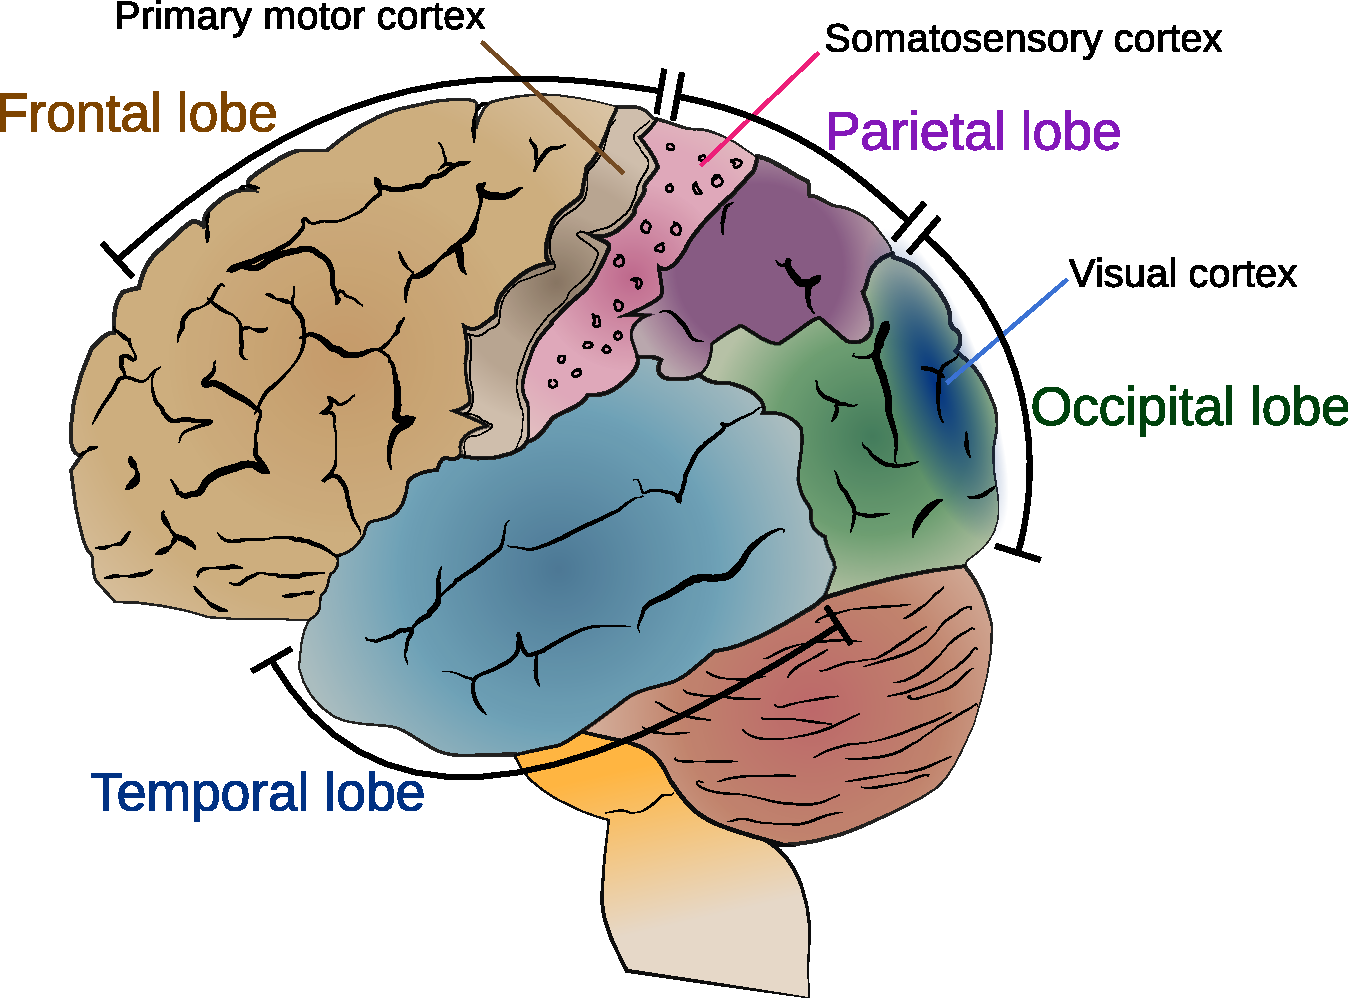
\includegraphics[scale=0.5]{images/Cerebrum_lobes}
    \caption[Functional Regions of the Cerebral Cortex]{Functional Regions of the Cerebral Cortex (Adapted from \href{http://en.wikipedia.org/wiki/File:Cerebrum_lobes.svg}{Wikipedia})}
    \label{fig:brain_parts}
\end{figure}
}

\mysubsubsection{Neurons}

\par{
    Neurons or nerve cells are the core components of the brain. There are
    approximately 10\textsuperscript{11} neurons in the human brain \citep{kandel_principles_2013}
    forming complex interconnected networks to produce human behavior.

\begin{figure}[ht]
    \centering
    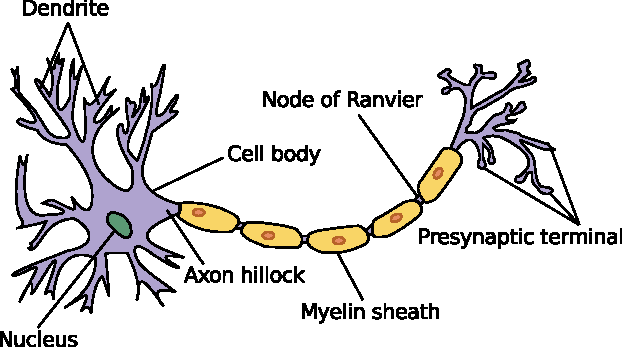
\includegraphics[scale=0.9]{images/neuron}
    \caption[The Structure of a Neuron]{The Structure of a Neuron (Adapted from \href{http://commons.wikimedia.org/wiki/File:Neuron.svg}{Wikipedia})}
    \label{fig:neuron}
\end{figure}
}

\par{
    A typical neuron is composed of four regions: The cell body or soma, dendrites, axon
    and presynaptic terminals (Figure ~\ref{fig:neuron}).
}
\par{
    The cell body, surrounded by a membrane made of a lipid bilayer, is the center
    of the neuron containing the nucleus which is responsible for protein synthesis.
    A number of short branches called \emph{dendrites} extend from the cell body. The function
    of dendrites is to receive incoming signals sent by other neurons. In contrast to having
    multiple dendrites for input, neurons have a single tubular output extension called \emph{axon}.
    This single axon branches out into extremities known as \emph{presynaptic terminals} which
    transmit the electrical signal to the (postsynaptic) dendrites of other neurons (postsynaptic cells)
    using special chemicals called \emph{neurotransmitters}. The zone where these presynaptic terminals
    and postsynaptic dendrites communicate with the help of neurotransmitters is called the \emph{synapse}.
    An axon has the ability to carry signals over distances
    between \emph{0.1mm} and \emph{2m} \citep{kandel_principles_2013}.
}
\par{
    \nomenclature{AP}{Action Potential}
    \begin{figure}[ht]
        \centering
        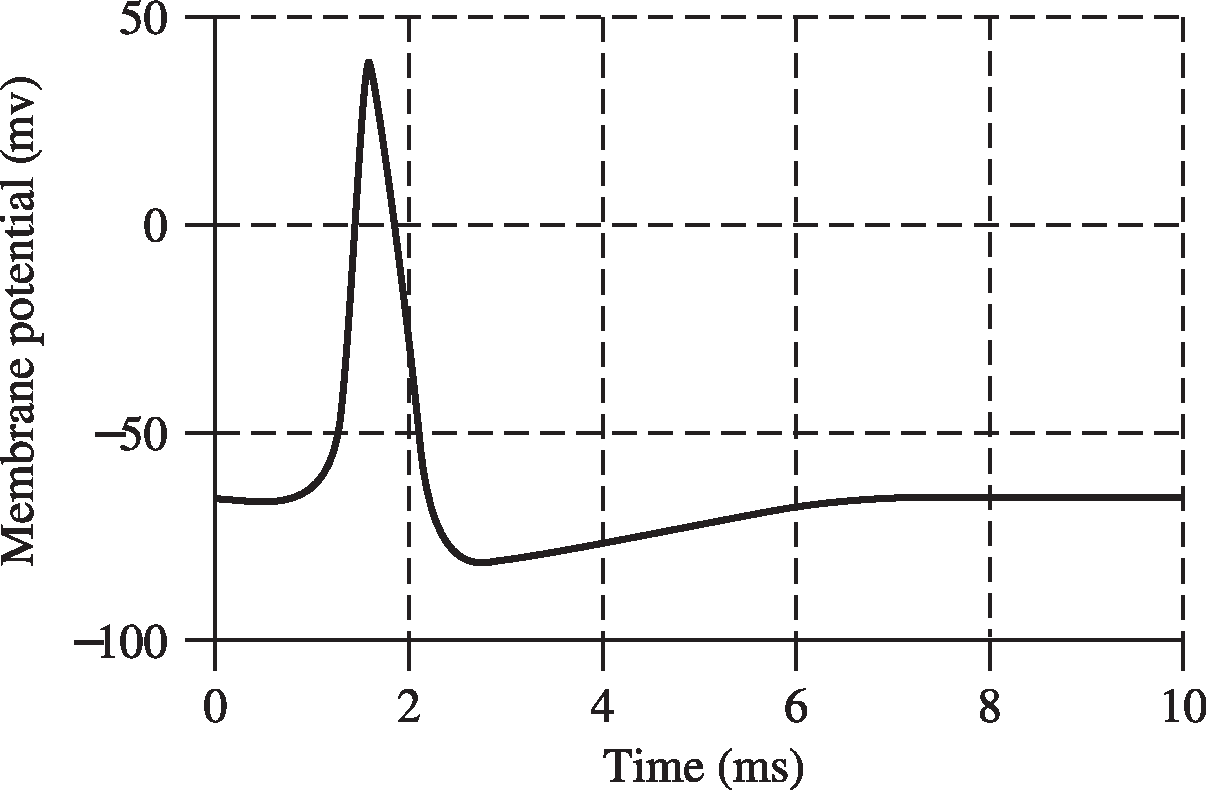
\includegraphics[scale=0.4]{images/ap}
        \caption[Action Potential]{Action Potential. \citep{sanei_eeg_2008}}
        \label{fig:action_pot}
    \end{figure}
    An action potential (AP), the electrical signal conducted through the neurons,
    is initiated at the initial part of the axon and propagates to the synapse.
    The generation of APs is an electrochemical phenomenon involving the protein
    structures found in the cell membrane called ion pumps and ion channels.
    More precisely, an AP is a temporary change in the membrane potential which
    normally rests at around \emph{-70 mV}, produced by an exchange of ions through the
    ion channels embedded in the cell membrane. This exchange is actually
    caused by an incoming stimulus reaching the dendrites of the neuron.
    Once this temporary change reaches a threshold potential around \emph{-55 mV}, an action potential is triggered
    (Figure ~\ref{fig:action_pot}): A sudden rise in the membrane potential (depolarization) often
    reaching around \emph{+30 mV} (\textasciitilde\emph{+100 mV} deflection from the resting
    potential) followed by a symmetrical fall (repolarization) ending below the resting potential
    at around \emph{-90 mV} (hyperpolarization). The membrane returns to its resting
    potential after this short (a few milliseconds) hyperpolarization phase.
}
\par{
    The brain receives, analyzes and carries information with the help of APs.
    An important functional characteristic of the brain is that the specificity
    of an information is not defined by the form of the signal but by the pathway
    the signal travels in the brain. It is the interpretation of signal patterns
    and pathways which leads to the sensation of several external stimuli \citep{kandel_principles_2013}.
}

\mysubsection{Measuring Brain Activity}
\par{
    \nomenclature{EEG}{Electroencephalography}
    \nomenclature{MEG}{Magnetoencephalography}
    \nomenclature{ECoG}{Electrocorticography}
    \nomenclature{fMRI}{Functional Magnetic Resonance Imaging}
    \nomenclature{fNIRS}{Functional Near-Infrared Spectroscopy}
    A BCI requires a method for observing the brain activity produced during
    various cognitive paradigms. There exists several methods (Table ~\ref{table:imaging_methods}) for sensing
    this activity each with its own pros and cons. We can categorize available
    methods in terms of the \emph{invasiveness} and the \emph{neurophysiological}
    origin of the measured activity.
}
\par{
    Two other parameters defined below are also important to
    assess the applicability of the technique in the BCI field:
    \begin{itemize}
        \item \emph{Temporal resolution} is the smallest time period of neural activity
            that can be reliably detected by the method.
        \item \emph{Spatial resolution} is the smallest neuronal area that can be
            reliably detected by the method.
    \end{itemize}
}
\mysubsubsection{Invasiveness}
\par{
    Invasiveness is a measure of how deep is a sensor going through the skin.
    Electroencephalography (EEG), magnetoencephalography (MEG), functional magnetic
    resonance imaging (fMRI) and functional near-infrared spectroscopy (fNIRS)
    are all \emph{non-invasive} methods as they record activity over the scalp.
}
\par{
    In contrast to non-invasive methods, \emph{invasive} methods need to implant
    microelectrodes inside the skull. In electrocorticography (ECoG), microelectrodes
    are placed on the surface of the cortex during a surgery, while intracranial (or
    intracortical) recordings use arrays of microelectrodes implanted inside the cortex (Figure ~\ref{fig:methods_eeg_ecog}\footnote{\url{https://wiki.ml.tu-berlin.de/wiki/NT/Courses/SS13_IL_AAND}}).

    Since ECoG electrodes stays on the surface of the cortex, it is sometimes referred to as a
    \emph{partially-invasive} technique \citep{demetriades_brain-machine_2010}.

    \begin{figure}[ht]
        \centering
        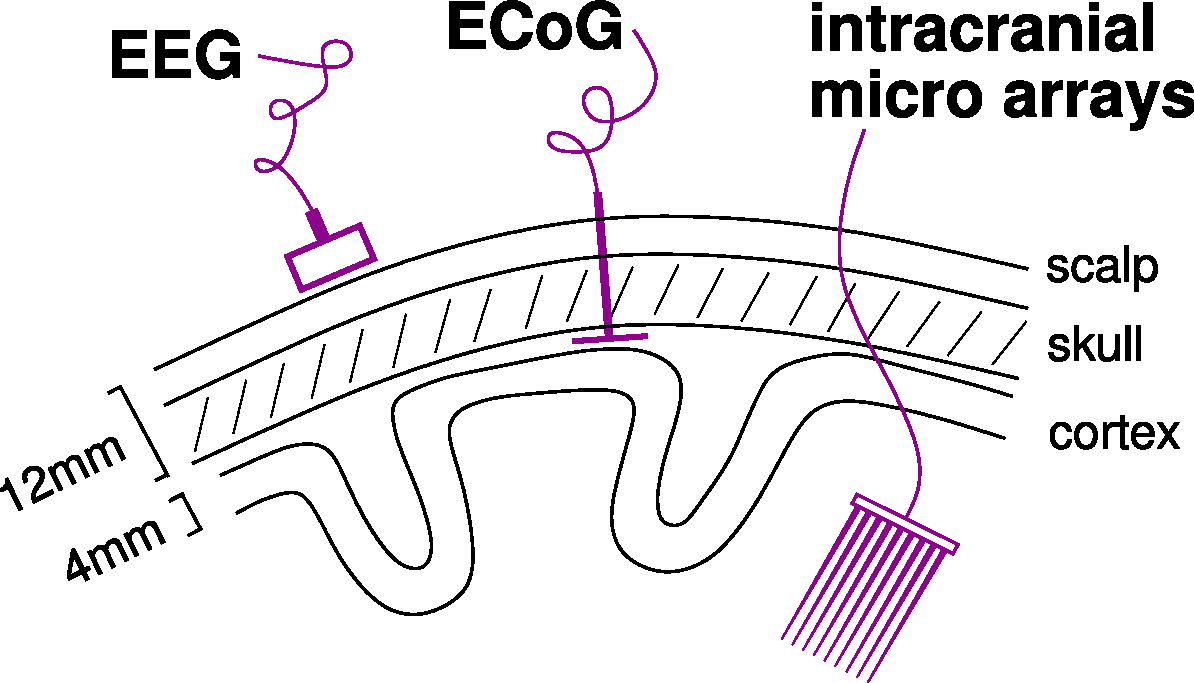
\includegraphics[scale=0.5]{images/eeg_vs_ecog}
        \caption[Invasiveness of EEG, ECoG and Intracranial Recordings]{Invasiveness of EEG, ECoG and Intracranial Recordings. (Courtesy of B. Blankertz)}
        \label{fig:methods_eeg_ecog}
    \end{figure}
}
\mysubsubsection{Neurophysiological Origin}
\par{
    The neurophysiological origin of the measured activity can either be electrophysiological
    or hemodynamic \citep{nicolas-alonso_brain_2012}.
}

\par{
    When neurons are activated, synaptic currents are produced within the dendrites.
    The magnetic and electrical fields generated by these currents constitute the
    so-called \emph{electrophysiological} activity. These activities can be measured
    invasively or non-invasively using MEG, EEG, ECoG and intracranial recordings.
}
\par{
    The body adjusts its blood flow to deliver oxygen and glucose to active tissues
    during physical activities. The rapid delivery of blood to active neurons in
    the brain is called the \emph{hemodynamic} response. These metabolic changes
    can be observed using imaging methods like fMRI and fNIRS. Since
    the hemodynamic response is the consequence of an augmented neuronal activity,
    these methods can be described as indirect methods \citep{nicolas-alonso_brain_2012}.
}
\mysubsubsection{Overview of Methods}
\par{
    Although each of the imaging methods mentioned before can be used in a BCI system,
    EEG surpasses other methods due to its high temporal resolution, portability,
    non-invasiveness and low cost. Consumer grade low cost EEG devices are also
    available making the technology more ubiquitous. The rest of this work will solely be focused on non-invasive EEG based BCI systems.
}
\par{
    fMRI and MEG require huge devices which are very expensive, non-portable and uncomfortable.
    ECoG and intracranial recordings can acquire high quality signals for BCI but they are not easily
    applicable due to their invasive nature. Once implanted, their signal quality
    can gradually become weaker in long term because of tissue reaction issues.
}
\par{
    fNIRS is recently gaining popularity for portable and non-invasive BCI design
    among researchers (\citealp{coyle_braincomputer_2007}; \citealp{pfurtscheller_hybrid_2010}; \citealp{fazli_enhanced_2012}).
    Although it has a low temporal resolution; the ease of installation over the
    scalp and its simplistic electronic design will probably make it an even more
    popular acquisition technique in the future years.

\begin{table}
    \footnotesize
    \centering
    \caption[Comparison of Brain Imaging Methods]{Comparison of Brain Imaging Methods \citep{nicolas-alonso_brain_2012}}
    \begin{tabular}{llllll}
        \hline
        \textbf{Method} &
        \textbf{\vtop{\hbox{\strut Temporal}\hbox{\strut Resolution}}} &
        \textbf{Spatial Resolution} &
        \textbf{Invasiveness} &
        \textbf{Activity} &
        \textbf{Portability} \\ \hline
        EEG             & \textasciitilde 0.05s & \textasciitilde 10mm  & Non-invasive & Electrical & Portable \\ \hline
        MEG             & \textasciitilde 0.05s & \textasciitilde 5mm   & Non-invasive & Magnetic & Non-portable \\ \hline
        ECoG            & \textasciitilde 0.003s & \textasciitilde 1mm  & Invasive & Electrical & Portable \\ \hline
        Intracortical   & \textasciitilde 0.003s & \textasciitilde 0.05mm - 0.5mm & Invasive & Electrical & Portable \\ \hline
        fMRI            & \textasciitilde 1s & \textasciitilde 1mm  & Non-invasive & Hemodynamic & Non-portable \\ \hline
        fNIRS           & \textasciitilde 1s & \textasciitilde 5mm  & Non-invasive & Hemodynamic & Portable \\ \hline
    \end{tabular}
    \label{table:imaging_methods}
\end{table}
}

\mysubsection{Principles of EEG}

\mysubsubsection{Electrode Placement}
\par{
Human EEG is recorded using an internationally recognized electrode naming and placement
standard called 10-20 system \citep{jasper_ten_1958} (Figure ~\ref{fig:eeg_1020}).
This standard is based on the relationship between electrode locations and the underlying
area of the brain. A combination of a letter and a number is further used to identify each electrode location.
}

\begin{figure}[ht]
    \centering
    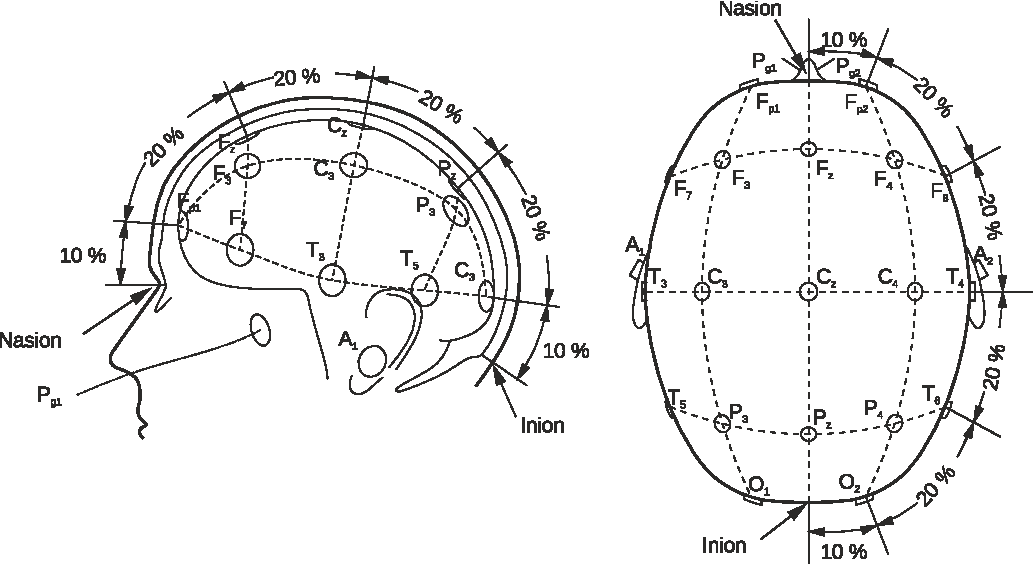
\includegraphics[scale=0.75]{images/10_20_bembook_redrawn}
    \caption[International 10-20 System]{International 10-20 System. \citep{nicolas-alonso_brain_2012}}
    \label{fig:eeg_1020}
\end{figure}

\par{
    The letters \emph{F, Fp, T, C, P} and \emph{O} respectively denotes \textbf{F}rontal, \textbf{F}ronto\textbf{P}olar
    (or \textbf{F}rontal \textbf{P}olar), \textbf{T}emporal, \textbf{C}entral, \textbf{P}arietal and
    \textbf{O}ccipital lobes. (Note that the \emph{C} letter is only meaningful as a notation to define the central line
    as the brain does not have an area called central lobe.) An A is used to refer to earlobes.
    Electrodes over the left hemisphere are suffixed with odd numbers and those over the right hemisphere
    are suffixed with even numbers. A \emph{"z"} instead of a number refers to an electrode placed on the midline, which
    is named the \emph{vertex}.

    \begin{figure}[ht]
        \centering
        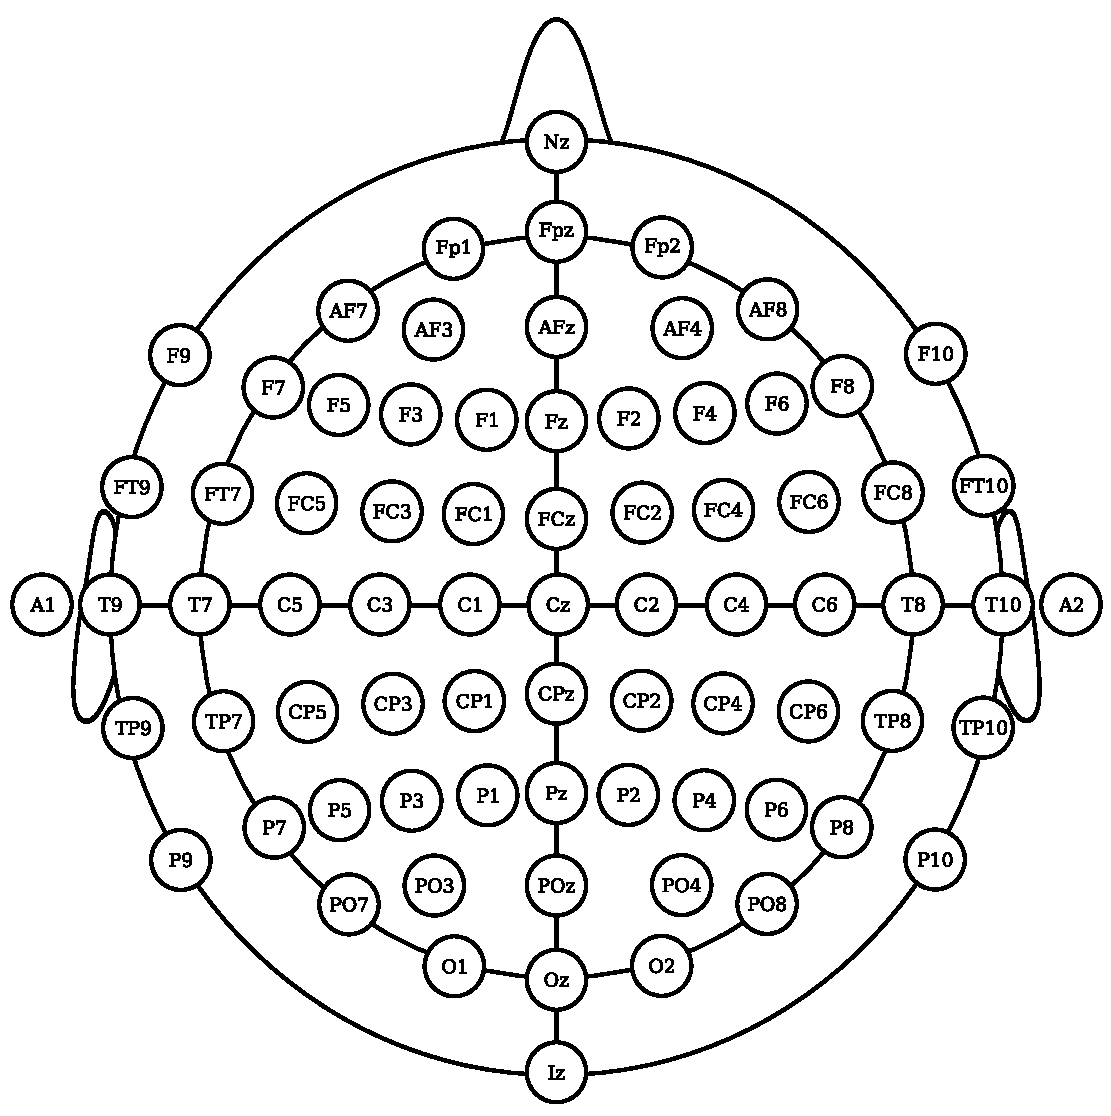
\includegraphics[scale=0.6]{images/10_20_extended}
        \caption[10-10 Combinatorial System]{10-10 Combinatorial System (Drawing courtesy of Marius 't Hart)}
        \label{fig:eeg_1020_comb}
    \end{figure}
}

\par{
    Two anatomical landmarks are used to define the longitudinal axis over the scalp: First, the \emph{Nasion (Ns or Nz)}, which is the
    depressed area between the eyes where the bridge of the nose joins the forehead; second, the \emph{Inion (In or Iz)}, which is
    indicated by a bump at the lower rear part of the skull. From these landmarks, Ns-In perimeters are divided into 10\% and 20\% intervals
    and electrode locations are fixed at those division points. Three other electrodes are placed on each hemisphere
    (F3,C3,P3 and F4,C4,P4) equidistantly from the already placed adjacent electrodes. The percentage of division intervals
    clearly reveals why the system is named after the term 10-20.
}

\par{
    Another widely used electrode placement schema is the full 10-10 combinatorial
    system \citeyearpar{guideline_1994} which is a sophisticated 10-20
    variant with more and more electrodes placed in between 10-20 locations
    (Figure ~\ref{fig:eeg_1020_comb}).
    %\footnote{Image courtesy of Marius 't Hart (\url{http://www.mariusthart.net/?e=200})}).
    New letters are introduced to define intermediate electrode sites: \emph{AF} is between Fp and F, \emph{FC} is between F and C,
    \emph{FT} is between F and T, \emph{CP} is between C and P, \emph{TP} is between T and P, and finally \emph{PO} is between P and O.
    The colored locations are actually T3, T4, T5 and T6 electrodes in 10-20 system but
    they are renamed to T7, T8, P7 and P8 in this modified schema.
}

\par{
    A new 10-5 extension with 345 electrodes was also proposed by \citet{oostenveld_five_2001} for high resolution EEG studies.
}

\mysubsubsection{Montage and Recording}
\begin{figure}
    \centering
    \begin{subfigure}{.5\textwidth}
        \centering
        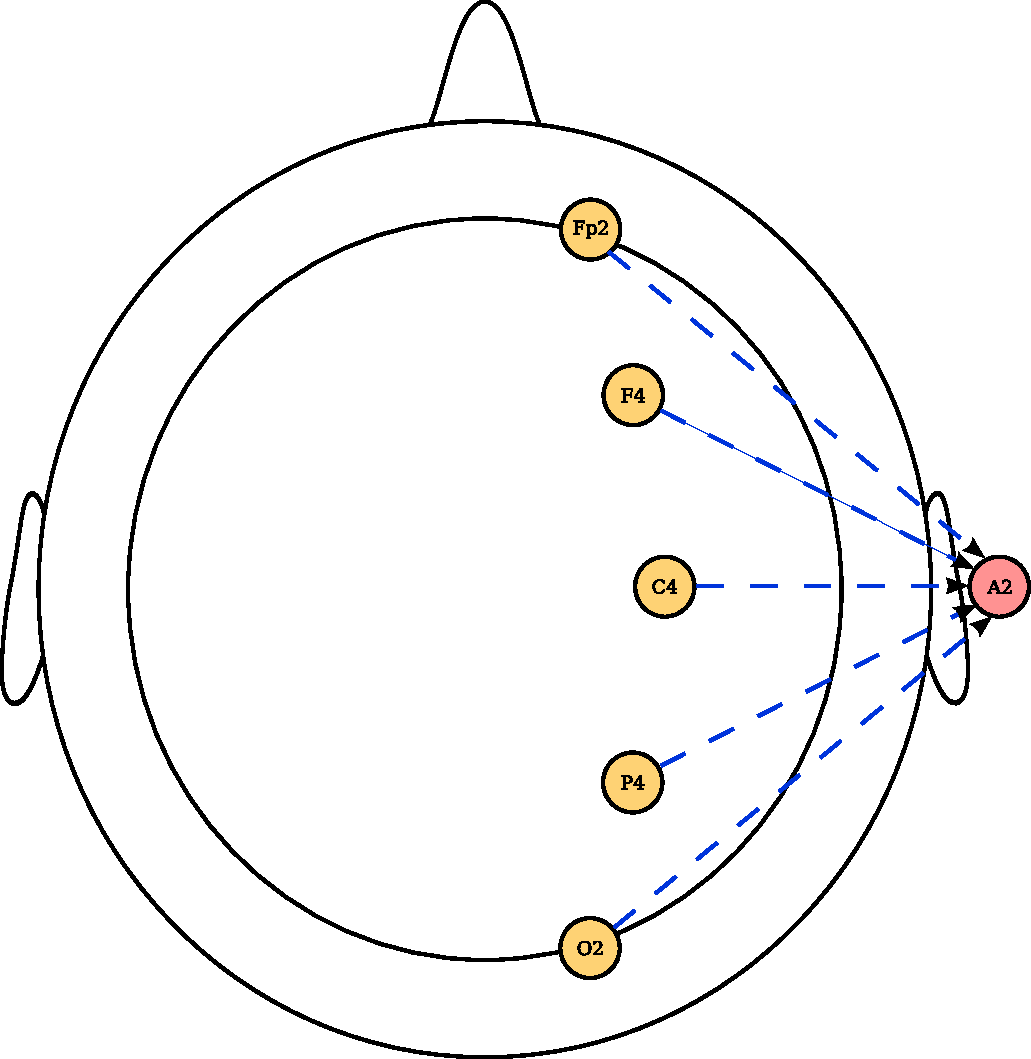
\includegraphics[scale=0.4]{images/unipolar_eeg}
        \caption{Referential Montage}
        \label{fig:referential_eeg}
    \end{subfigure}%
    \begin{subfigure}{.5\textwidth}
        \centering
        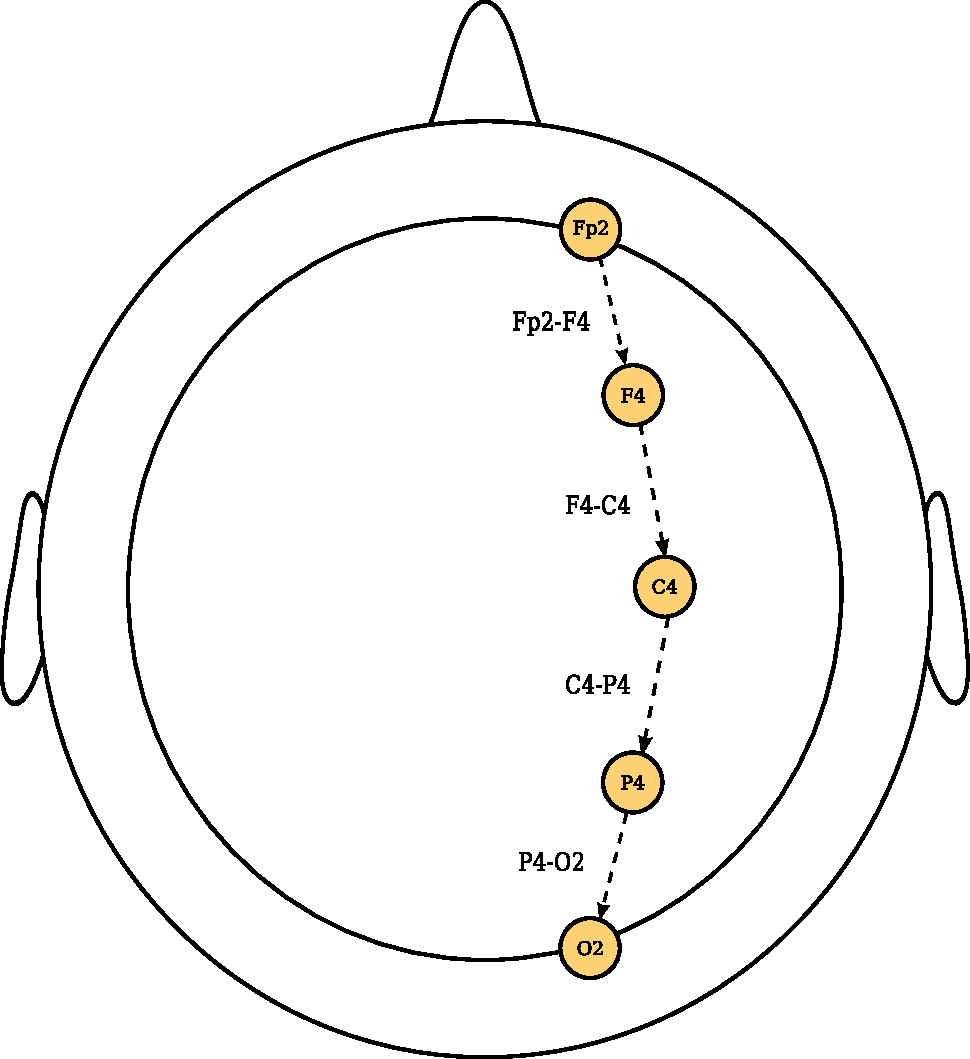
\includegraphics[scale=0.4]{images/bipolar_eeg}
        \caption{Bipolar Montage}
        \label{fig:bipolar_eeg}
    \end{subfigure}
    \caption{A Comparison of Referential and Bipolar Montages}
    \label{fig:ref_bipolar_eeg}
\end{figure}


\par{
    What is measured in EEG is defined as potential differences between pairs
    of electrodes placed on various scalp locations \citep{nunez_electric_2006}.
    One of the electrodes is generally called \emph{recording} or \emph{signal}
    electrode while the other is defined as the \emph{reference} electrode. It is
    important to note that although the adjective \emph{reference} seems to
    designate an electrode which captures an unchanging baseline/neutral signal,
    both electrodes actually record real and alternating brain signals \citep{wolpaw_brain-computer_2012}.
}
\par{
    \emph{Referential recording} refers to a montage where EEG is recorded
    between each recording electrode and a reference electrode with a fixed position (Figure ~\ref{fig:referential_eeg}).
    This is the montage generally used in cognitive studies and BCIs.
}
\par{
    In contrast, \emph{Bipolar recordings} measure potential differences between
    adjacent/very close electrodes: The reference electrode is not fixed at a
    specific location but varies according to the recording electrode (Figure ~\ref{fig:bipolar_eeg}).
}
\par{
    It is trivial to switch between montages with basic arithmetic operations once EEG is acquired and digitized.
    Re-referencing to another electrode is also possible at this stage.
}

\mysubsubsection{Electrode Types}
\par{
    There are basically two types of electrodes used for recording EEG: \emph{Passive} electrodes and
    \emph{active} electrodes.
}
\par{
    \emph{Passive} electrodes are tiny metal disks usually made of tin, gold, silver
    or silver/silver-chloride (Ag/AgCl) connected to an amplifier
    through electrical wires. The signal they acquire is then amplified in the
    external amplifier circuitry. Since brain signals acquired through the scalp
    have amplitudes ranging between 10-100uV \citep{sanei_eeg_2008}, higher amplitude noise sources like
    head movements, environmental factors and electrical line noise (A 50 or 60 Hz
    frequency signal depending on the country) have the risk to garble the signals as their
    amplitudes become even higher after amplification. To avoid this problem as much as
    possible, electrode cables must be short, shielded and fixed.
}
\par{
    A good contact between the scalp and the electrodes is also crucial to
    improve the signal-to-noise ratio of the acquired signals. A layer of conductive
    gel paste is generally applied before recordings to reduce the skin-electrode impedance (opposition to current).
    Unfortunately, the application of the gel paste is cumbersome, time consuming and
    leaves pasty residue that will not go away without washing. An easier and
    cleaner alternative to gel paste is to put sponge-like pads between the
    electrode and the scalp and to soak them with saline solution (e.g. salt and water).
    This sponge-saline approach is the one preferred in Emotiv's wireless
    EEG headsets. The obvious disadvantage of this method is that the impedance
    goes up as the sponges dry \citep{wolpaw_brain-computer_2012}.
}
\par{
    On the other hand, \emph{dry} electrodes
    that do not require the application of a conductive material is heavily
    researched to improve the ergonomics of EEG recordings (\citealp{popescu_single_2007}; \citealp{grozea_bristle-sensorslow-cost_2011}).
    These electrodes generally penetrate through the hair
    with their fiber-like electrode tips to increase the conductivity.
}
\par{
    \emph{Active} electrodes make use of a small built-in circuitry to amplify
    the signals before the transmission takes place. The preamplified brain signals
    are thus more robust against external noise sources mentioned above since
    the additive noises are not preamplified.
}
\par {
    \begin{figure}
        \centering
        \begin{subfigure}{.33\textwidth}
            \centering
            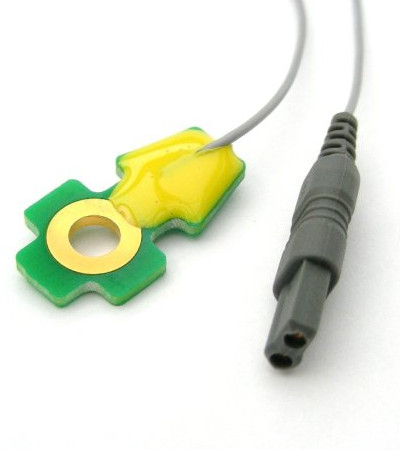
\includegraphics[height=4cm]{images/gtec_passive}
            \caption{}
            \label{fig:electrode_gtec}
        \end{subfigure}%
        \begin{subfigure}{.33\textwidth}
            \centering
            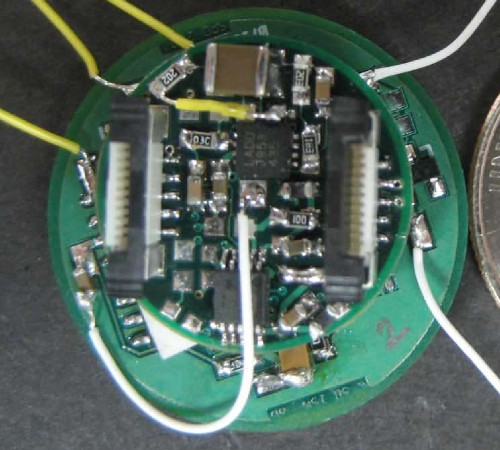
\includegraphics[height=4cm]{images/active_electrode}
            \caption{}
            \label{fig:electrode_active}
        \end{subfigure}%
        \begin{subfigure}{.33\textwidth}
            \centering
            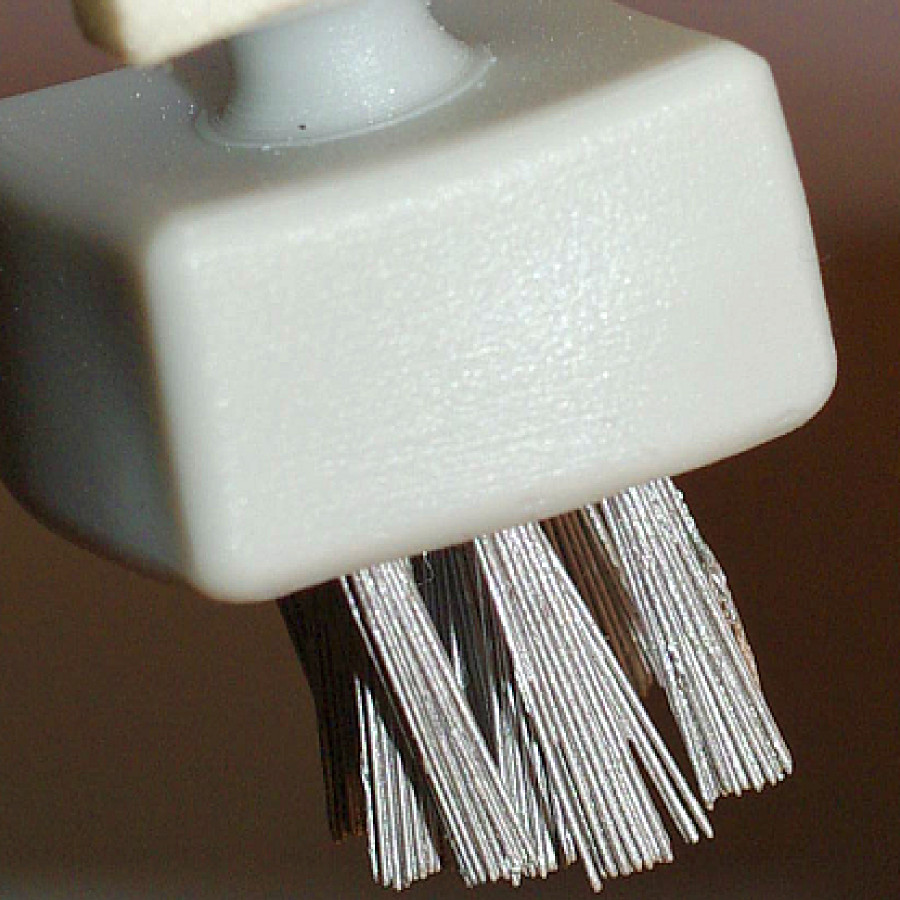
\includegraphics[height=4cm]{images/bristle_dry}
            \caption{}
            \label{fig:electrode_dry}
        \end{subfigure}
        \caption[Different Types of Electrode]{Different Types of Electrode: (a) A passive electrode by \emph{g.tec} (b) An active electrode \citep{sullivan_low-noise_2007} (c) A dry electrode prototype \citep{grozea_bristle-sensorslow-cost_2011}}
        \label{fig:diff_types_electrode}
    \end{figure}

    Passive electrodes are generally the preferred type of electrode in EEG recordings
    since they are simple to design and cheap to manufacture \citep{wolpaw_brain-computer_2012}
    compared to expensive and sophisticated active electrodes. A visual comparison
    of the mentioned sensor technologies can be seen in Figure ~\ref{fig:diff_types_electrode}.
}

\mysubsubsection{Brain Rhythms in EEG}
\par{
    The frequency (or spectral) content of EEG signals is generally divided into five frequency
    bands: Delta rhythm (0.1-3.5 Hz), theta rhythm (4-7.5 Hz), alpha rhythm (8-13 Hz),
    beta rhythm (14-30 Hz) and gamma rhythm (> 30 Hz) \citep{niedermeyer_electroencephalography:_2005}.
    A sixth one called mu rhythm (8-12 Hz) can be observed when motor neurons are in the idling
    state \citep{wang_practical_2010}. Although the frequency intervals of mu and
    alpha rhythms seem to overlap, alpha rhythm is observed over the visual cortex
    while the mu rhythm is prominent over the sensorimotor cortex.
}
    \par{
    \begin{figure}[ht]
        \centering
        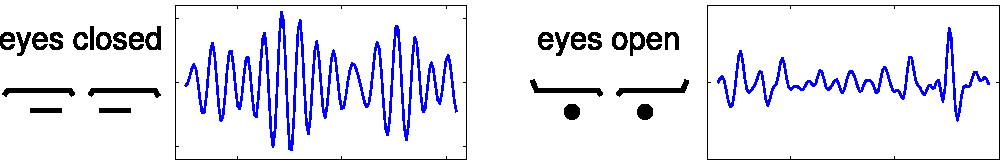
\includegraphics[scale=0.8]{images/alpha_eyes}
        \caption[Alpha Rhythm Over Oz]{Alpha Rhythm Over \emph{Oz} (Courtesy of B.Blankertz)}
        \label{fig:eeg_alpha}
    \end{figure}

    The observation or absence of these rhythmic activities is generally associated
    with external stimuli processing, sleep states, cognitive actions or pathological
    findings. For example, an alpha rhythm around 10 Hz over the visual cortex
    is attenuated during visual processing, e.g. while the eyes are open (Figure ~\ref{fig:eeg_alpha}\footnote{\url{https://wiki.ml.tu-berlin.de/wiki/NT/Courses/SS13_IL_AAND}}).
}

\mysubsection{BCI Paradigms}
\par{
    There are several paradigms used in BCI design for extracting control information
    out of the brain. A BCI system is defined as active/endogenous or
    reactive/exogenous based on the underlying cognitive mechanism of the paradigm used.
}
% FIXME: Explain later
%\mysubsubsection{Event-Related Potentials}
%\par{
%    \nomenclature{ERP}{Event-Related Potential}
%    Event-Related potentials (ERP) are defined as potential changes in
%    neural activity associated with specific cognitive events \citep{luck_introduction_2005}.
%}

%%%%%%%%%%%%%%%%%%%%%%%%%%%%%%%%%%%%%%%%%%%%%%%%%%%%%%%%%%%
\newpage
\mysubsubsection{Steady-State Visual Evoked Potentials}
\par{
    \nomenclature{VEP}{Visual Evoked Potential}
    \nomenclature{SSVEP}{Steady-State Visual Evoked Potential}
    \begin{figure}[ht]
        \centering
        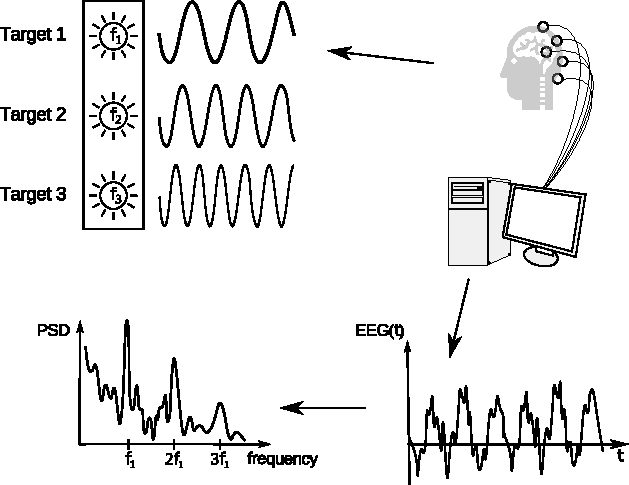
\includegraphics[width=0.7\textwidth]{images/ssvep_diagram}
        \caption[Diagram of a SSVEP BCI]{Diagram of a SSVEP BCI \citep{chumerin_decoding_2012}}
        \label{fig:eeg_ssvep_bci}
    \end{figure}
    A steady-state visual evoked potential (SSVEP) is an exogenous response
    to a repetitive visual stimuli which usually oscillates at the fundamental
    and harmonic frequencies of the flickering stimulus \citep{wu_stimulator_2008}.
}
\par{
    In a typical SSVEP BCI setup, targets are generally represented to the user
    in a flickering fashion be it an LED light, a pattern on a CRT or LCD screen, etc (Figure ~\ref{fig:eeg_ssvep_bci}).
    The type of stimulation device, the color and the shape of the stimulus,
    the frequency band of the oscillation rate and the phase between stimuli
    are characteristics of the light stimuli which can affect the SSVEP \citep{zhu_survey_2010}.
}
\par{
    Since SSVEP is a response to a repetitive visual stimulus, it is prominent
    and observable through the occipital locations near the primary visual
    cortex \citep{herrmann_human_2001}.
}

%%%%%%%%%%%%%%%%%%%%%%%%%%%%%%%%%%%%%%%%%%%%%%%%%%%%%%%%%%%
\newpage

\mysubsubsection{Slow Cortical Potentials}
\par{
    \nomenclature{SCP}{Slow Cortical Potentials}
    Slow Cortical Potentials (SCP) are voltage changes in EEG which occur
    slowly over time, e.g. between 0.5-10 seconds \citep{wolpaw_brain_2010}.
    The fact that these slow potentials can be consciously regulated
    by healthy and paralyzed people, makes SCP a choice for BCI design
    (\citealp{birbaumer_thought_2000}; \citealp{hinterberger_brain-computer_2004}; \citealp{birbaumer_breaking_2006}).
}
\par{
    SCP-based BCIs are active/endogenous systems as the user has to voluntarily adjust
    the polarity (negative/positive) of their slow potentials according to some neurofeedback protocol \citep{jackson_neural_2010}.
    They can be used to select between binary targets (target selection) since the control signal is a bi-state
    negative/positive shift in slow potentials. This binary selection can also be extended
    to a speller application in which a letter is recursively selected by halving
    the alphabet in each step \citep{birbaumer_thought_2000}.
}

\mysubsubsection{Sensorimotor Rhythms}
\par{
    \nomenclature{SMR}{Sensorimotor Rhythms}
    \nomenclature{MI}{Motor Imagery}
    \begin{figure}[ht]
        \centering
        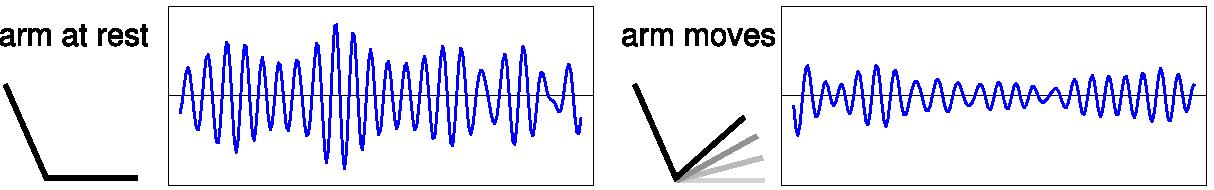
\includegraphics[scale=0.7]{images/motor_imagery}
        \caption[Mu Rhythm Over Sensorimotor Cortex]{Mu Rhythm Over Sensorimotor Cortex (Courtesy of B.Blankertz)}
        \label{fig:eeg_motor_imagery}
    \end{figure}

    Sensorimotor rhythms (SMR) are idling (rhythms observable while the
    user is at rest) mu and beta rhythms prominent over the sensorimotor cortex which are desynchronized
    (suppressed) with the activation of the motor system like the movement
    of hands or foot \citep{sellers_bcis_2010}. These changes not only happen
    with the actual movement but also with the imagination of movement, e.g. motor imagery (MI) \citep{mcfarland_braincomputer_2006}.
    The terms SMR, MI or mu rhythm can be used interchangeably to define this
    type of BCI.
}
%%%%%%%%%%%%%%%%%%%%%%%%%%%%%%%%%%%%%%%%%%%%%%%%%%%%%%%%%%%
\newpage

\par{
    \begin{figure}[ht]
        \centering
        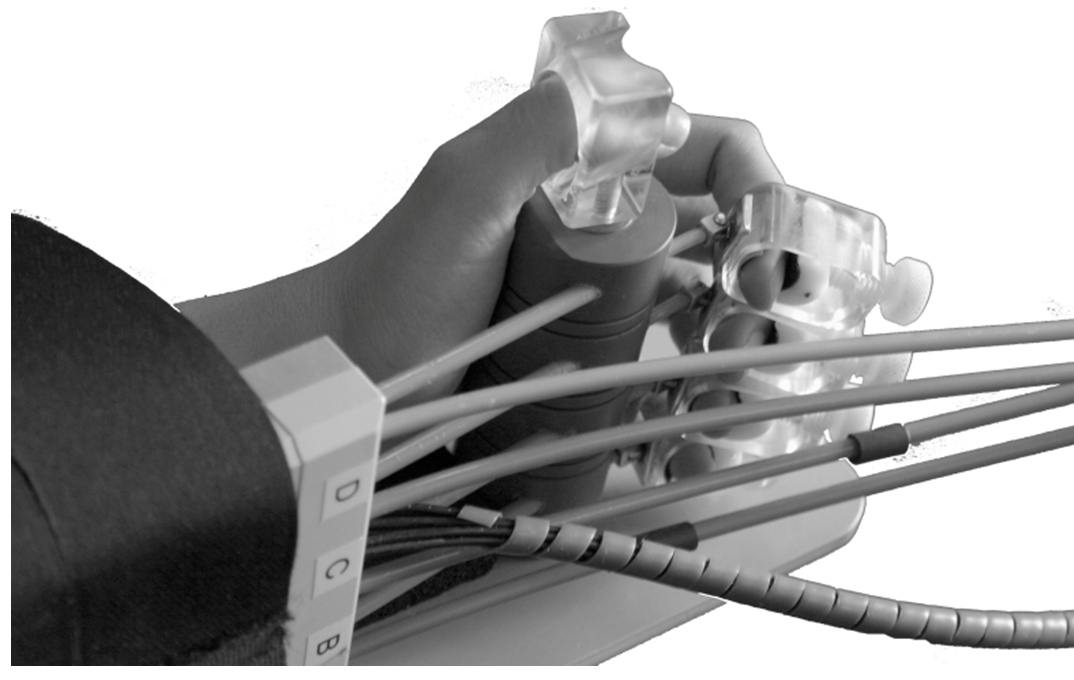
\includegraphics[width=0.6\textwidth]{images/bci_hand_rehab}
        \caption[Hand Orthosis for Neurorehabilitation]{Hand Orthosis for Neurorehabilitation \citep{ramos-murguialday_proprioceptive_2012}}
        \label{fig:motor_orthosis}
    \end{figure}
    SMR-based BCIs are active/endogenous systems as the user has to initiate/plan/imagine
    a movement to adjust their EEG rhythms. SMR-based BCIs are used in cursor control
    applications to select between targets
    (\citealp{wolpaw_eeg-based_1991}; \citealp{wolpaw_wadsworth_2003}; \citealp{vaughan_wadsworth_2006}),
    neurorehabilitation (Figure ~\ref{fig:motor_orthosis}) applications (\citealp{prasad_using_2009}; \citealp{ramos-murguialday_proprioceptive_2012};
    \citealp{ortner_human-computer_2013}), orthotics and prosthetics control (\citealp{guger_prosthetic_1999}; \citealp{pfurtscheller_motor_2001}).
}



%%%%%%%%%%%%%%%%%%%%%%%%%%%
%% MATERIALS AND METHODS %%
%%%%%%%%%%%%%%%%%%%%%%%%%%%
\clearpage
\vspace*{-0.35cm}
\mysection{MATERIALS AND METHODS}

\mysubsection{Materials}
\par{
    There exists 3 important hardware components of our embedded BCI
    design: an EEG headset for brain signal acquisition, an embedded
    computer to manage all kinds of interaction between the
    individual parts of the BCI and finally an external actuator to reflect
    the choices of the BCI user to the environment, e.g. the arms of a humanoid robot
    for this study.
}
\mysubsubsection{Kondo KHR-3HV Humanoid Robot}
\par{
    \begin{figure}[ht]
        \centering
        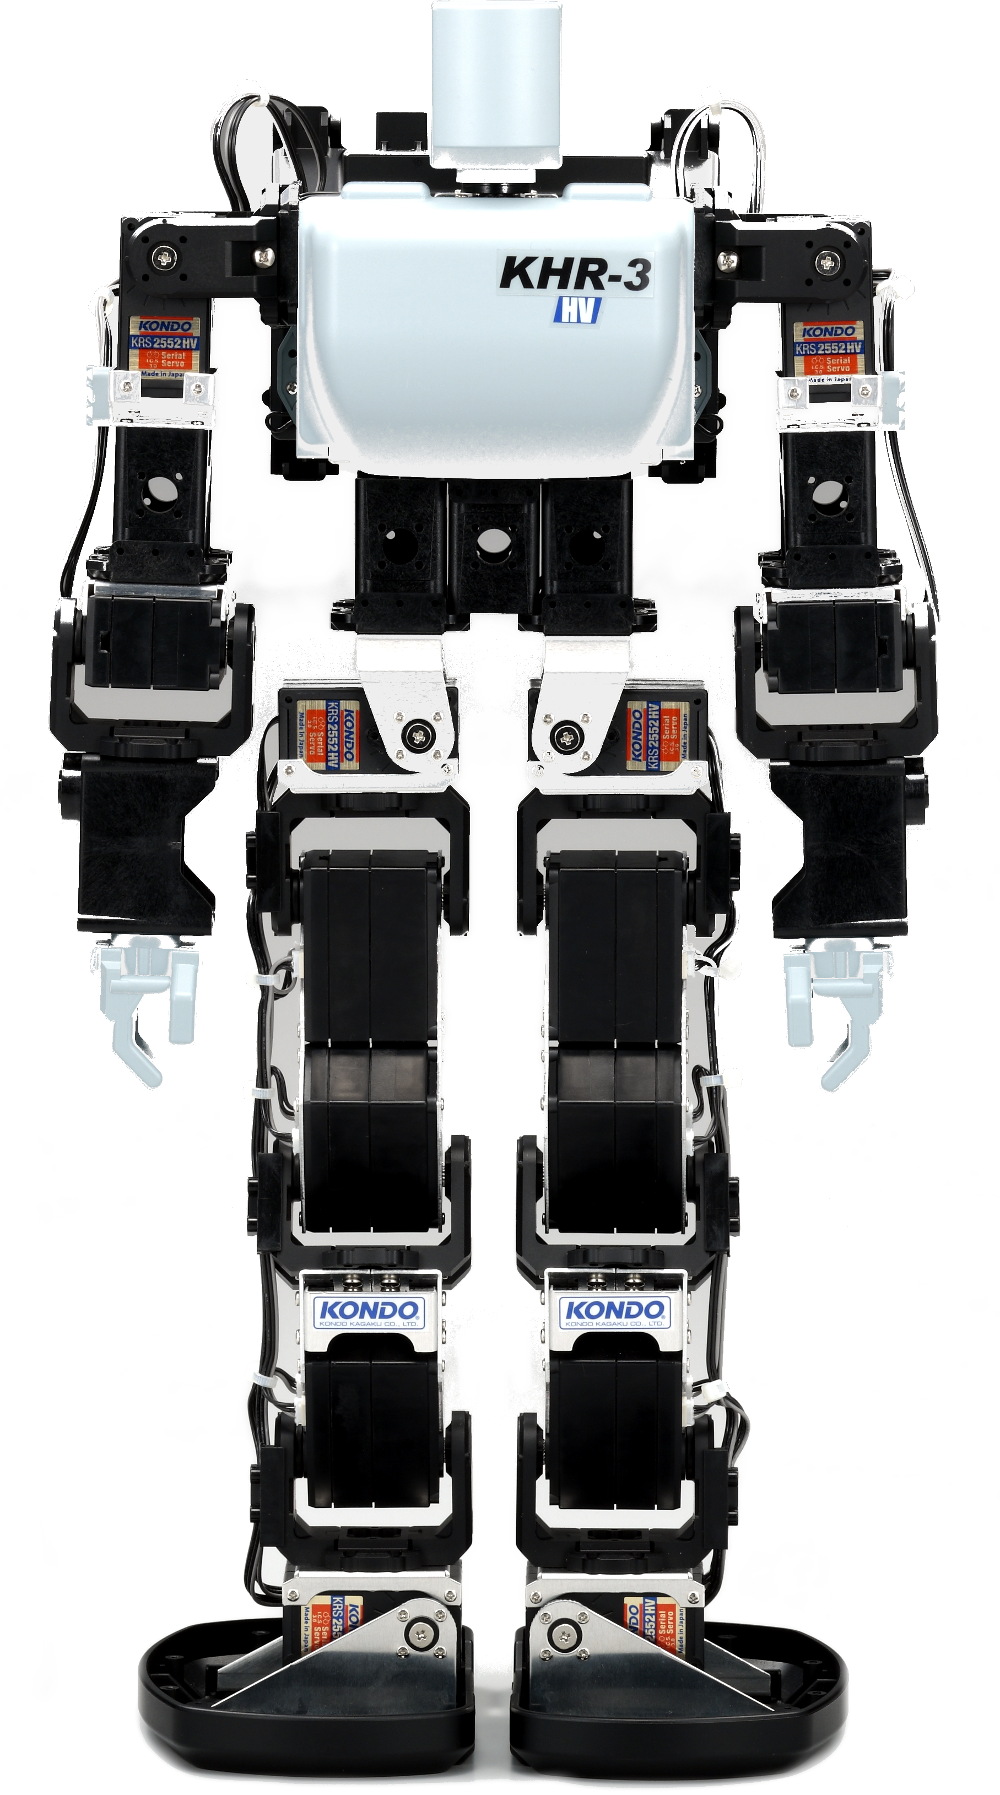
\includegraphics[scale=0.7]{images/kondo}
        \caption{Kondo KHR-3HV Humanoid Robot}
        \label{fig:kondo}
    \end{figure}
    Kondo KHR-3HV is a 17 degrees of freedom humanoid robot manufactured by
    \emph{Kondo Kagaku} (Figure ~\ref{fig:kondo}). The RCB-4 microcontroller of the robot has the
    ability to drive up to 35 serial servos. The board is also equipped with
    several I/O ports to extend the robot with sensors and other add-ons.
}
\par{
    The motions for KHR-3HV is designed and programmed into the microcontroller
    using a Windows application called \emph{Heart-to-Heart}. All communication
    between the computer and the robot (both for programming and controlling)
    is realized over a serial USB dongle. Once the motions are designed and written
    into the microcontroller using the proprietary software,
    it is possible to play those preprogrammed motions and
    control individual servos separately with the open-source and community
    contributed \emph{libkondo4} library\footnote{\url{https://bitbucket.org/vo/libkondo4}}.
    The library has also language bindings to allow controlling the robot using Python and Java.
}

\mysubsubsection{BeagleBone Black}

\par{
    \nomenclature{BBB}{BeagleBone Black}
    BeagleBone Black (BBB) is a 45\$ single board computer released in 2013. It has 1GHz TI AM3359 Sitara ARM Cortex-A8 microprocessor,
    512MB DDR3 memory, 3D accelerated PowerVR SGX530 graphical processing unit (GPU) with HDMI output, onboard 2GB embedded MMC (eMMC)
    flash storage pre-loaded with Ångström Linux distribution (Figure ~\ref{fig:bbb}). Along with a single USB 2.0 host port and 10/100 RJ45 Ethernet port for
    general purpose connectivity, the board also provides a wide variety of low-level expansion interfaces:
    66xGPIO, 5xUART, 8xPWM, 8xADC, 2xI\textsuperscript{2}C, SPI and CAN. A 4 port bus powered external USB hub is used for
    increasing the number of USB devices that can be connected to the BBB.
}

\begin{figure}[ht]
    \centering
    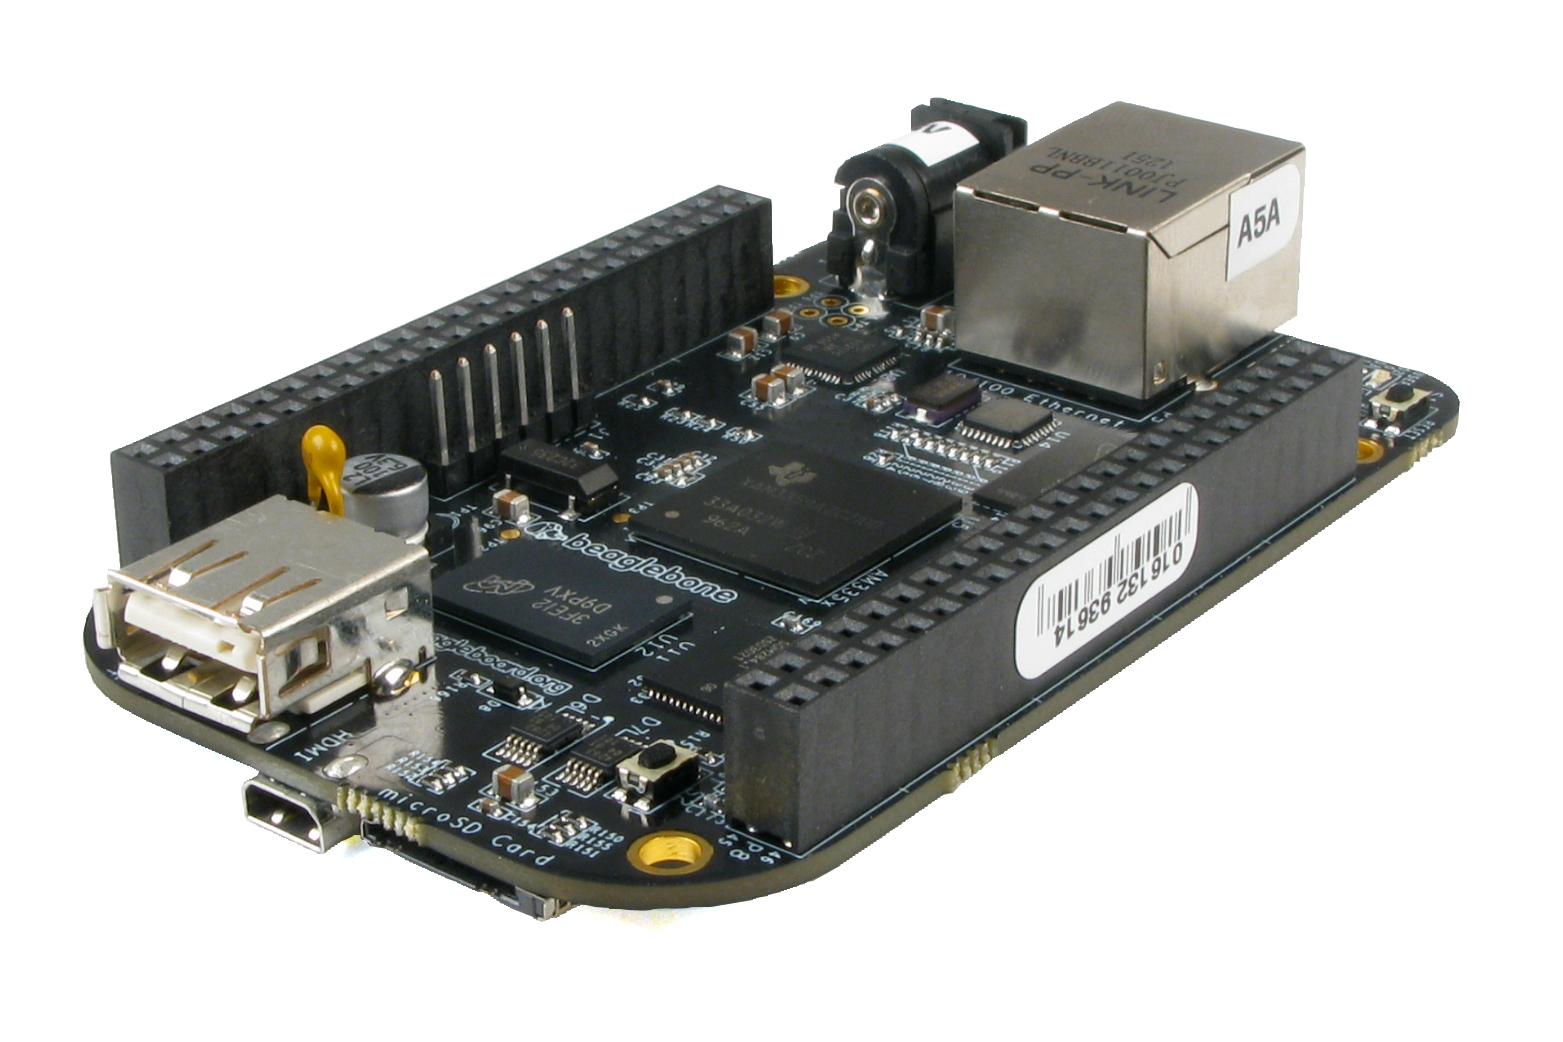
\includegraphics[width=0.55\textwidth]{images/bbb}
    \caption{BeagleBone Black Single-board Computer}
    \label{fig:bbb}
\end{figure}

\par{
    We first installed Ubuntu to an 8GB micro SD card as it is a widely adopted Linux distribution with a rich software repository.
    A rich software repository is important for avoiding manual compilation/installation of several tools and libraries,
    which in turn decreases the time needed to start experimenting with the BCI system. We also disabled
    several unused system services to avoid wasting processor and memory resources.
}

\mysubsubsubsection{Programmable Realtime Unit}
\par{
    \nomenclature{PRU}{Programmable Realtime Unit}
    Although the Cortex-A8 processor is powerful, real-time control of high-speed external hardware
    and high precision tasks can be affected by OS latencies. BBB improves the
    situation by providing two programmable realtime units (PRU) optimized to perform embedded tasks
    with hard realtime constraints. The PRUs have:
    \begin{itemize}
        \item Two 32-bit RISC cores running at 200MHz (Each instruction completes in 5ns)
        \item 8KB data memory and 8KB instruction memory
        \item 12KB shared memory
        \item A small instruction set
    \end{itemize}
    It is sometimes possible to encounter delays in OS scheduling while EEG
    acquisition and SSVEP stimulation are both running simultaneously. This can negatively
    impact the precision of flickering intervals causing the BCI to perform badly.
    Offloading SSVEP stimulation or any other high precision tasks to the
    PRU can resolve jitters and delays as PRU is a distinct
    microcontroller unit which is completely decoupled from the main CPU of the device.
}
\par{
    By now, the PRU can only be programmed using assembly language. A helper library
    for C and Python is available to launch and terminate custom programs written for the PRU.
    It is also possible to share data between the PRU and the CPU using shared memory.
}

\mysubsubsection{Emotiv EEG}

\par{
    %\begin{figure}[ht]
    %    \centering
    %    \includegraphics[width=0.5\textwidth]{images/emotiv}
    %    \caption{Emotiv EEG Headset}
    %    \label{fig:emotiv_eeg_headset}
    %\end{figure}
    %\begin{figure}[ht]
    %    \centering
    %    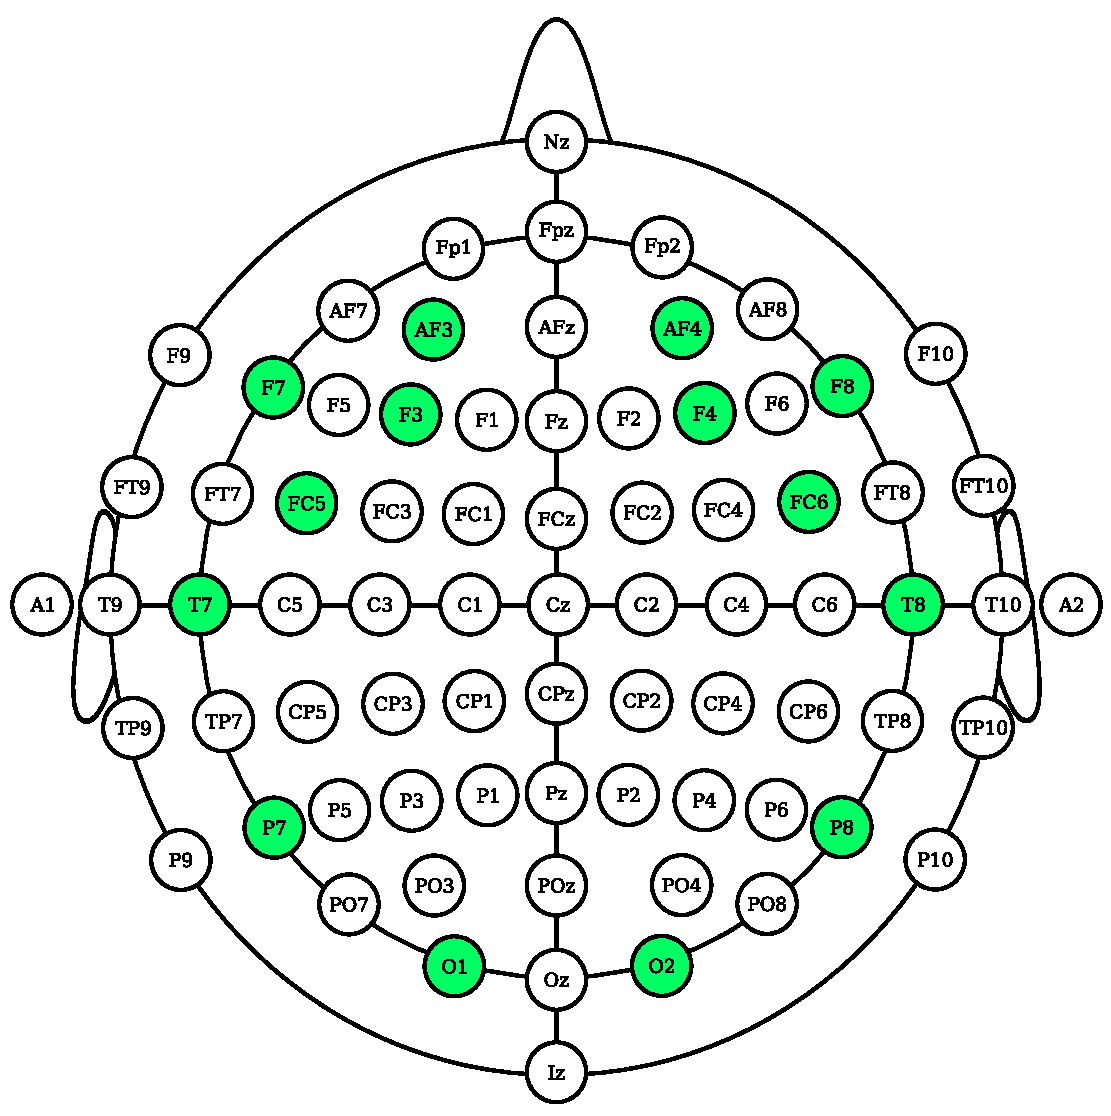
\includegraphics[scale=0.5]{images/10_20_emotiv}
    %    \caption{Emotiv EEG Electrode Locations}
    %    \label{fig:emotiv_eeg_1020}
    %\end{figure}
    \begin{figure}
        \centering
        \begin{subfigure}{.45\textwidth}
            %\centering
            \vspace*{2.55cm}
            \includegraphics[height=5cm]{images/emotiv}
            \caption{Emotiv EEG Headset}
            \label{fig:emotiv_eeg_headset}
        \end{subfigure}%
        \begin{subfigure}{.55\textwidth}
            \centering
            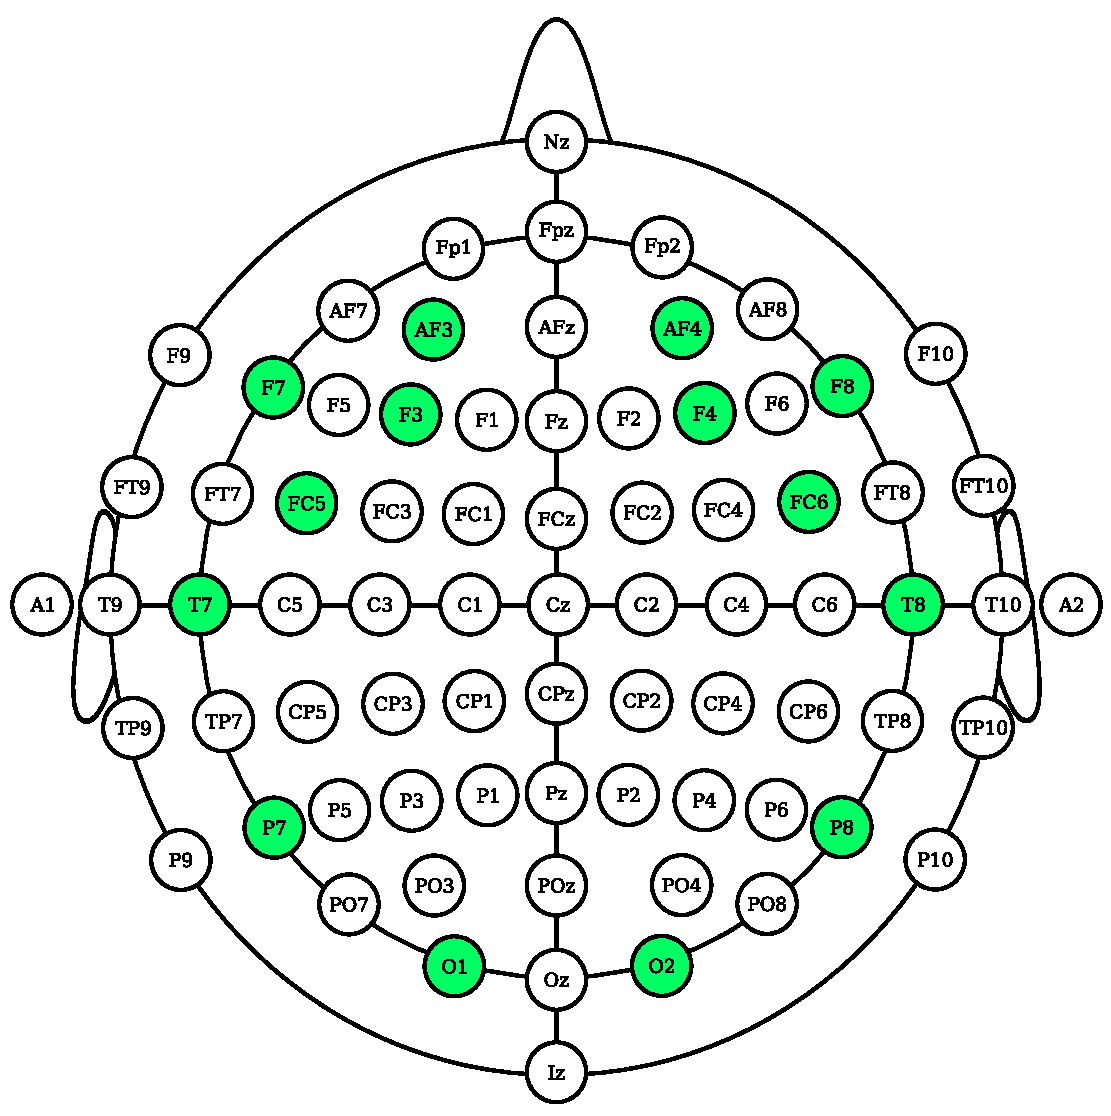
\includegraphics[scale=.4]{images/10_20_emotiv}
            \caption{Electrode Locations}
            \label{fig:emotiv_eeg_1020}
        \end{subfigure}
        \caption{Emotiv EEG Headset and Electrode Locations}
        \label{fig:emotiv_eeg_headset_locations}
    \end{figure}

    Emotiv EEG (Figure ~\ref{fig:emotiv_eeg_headset}) is a battery-powered, wireless consumer headset which can
    acquire 14 channels (Figure ~\ref{fig:emotiv_eeg_1020}) of EEG signal. Although Emotiv EEG is primarily
    researched for gaming and entertainment applications (\citealp{van_vliet_designing_2012}; \citealp{chumerin_steady-state_2013}),
    several research activities are targeting it to assess and exploit its usability for
    assistive BCI applications (\citealp{liu_implementation_2012}; \citealp{badcock_validation_2013}; \citealp{caglayan_humanoid_2013}; \citealp{guneysu_ssvep_2013}; \citealp{choi_low-cost_2013}).
}
\par{
    \begin{table}
        \footnotesize
        \centering
        \caption{Technical Specifications of Emotiv EEG Headset}
        \begin{tabular}{ll}
            \hline
            Number of channels & 14 (+ CMS/DRL references, P3/P4 locations) \\ \hline
            Channel names & AF3, F7, F3, FC5, T7, P7, O1, O2, P8, T8, FC6, F4, F8, AF4 \\ \hline
            Sampling method & Sequential sampling, single ADC \\ \hline
            Sampling rate & 128 SPS (2048 Hz Internal) \\ \hline
            Resolution & 14 bits 1 LSB = 0.51uV \\ \hline
            Bandwidth & 0.2-45Hz, digital notch filters at 50Hz and 60Hz \\ \hline
            Filtering & Built-in digital 5th order Sinc filter \\ \hline
            Dynamic range (input referred) & 8400uV (pp) \\ \hline
            Coupling mode & AC coupled \\ \hline
            Connectivity & Proprietary wireless, 2.4GHz band \\ \hline
            Battery life & 12 hours (typical) \\ \hline
            Impedance measurement & Real-time contact quality using patented system \\ \hline
        \end{tabular}
        \label{table:emotiv_eeg_specs}
    \end{table}
    The headset internally applies a
    notch filter (At line frequency 50/60Hz) and a 5\textsuperscript{th} order band-pass filter (0.2-45Hz)
    to the signal. Although the internal sampling rate of the headset is 2048Hz, the device
    downsamples the signal to 128Hz before sending them to the computer. Full technical specifications found in the
    manufacturer's website\footnote{\url{http://www.emotiv.com/eeg/download_specs.php}} are summarized in Table ~\ref{table:emotiv_eeg_specs}.
}
\par{
    Emotiv EEG uses a fixed reference electrode pair around P3/P4 region as the default
    reference location. The manufacturer also provided an alternative reference electrode
    pair right behind the ears. It is possible to switch to that reference location
    by removing the plastic rubber pads and inserting the spongy pads to those spots
    instead of the default reference locations\footnote{\url{http://emotiv.com/ideas/forum/forum12/topic2507}}.
}

\mysubsubsubsection{Official Software Development Kit (SDK)}

\par{
    Emotiv provides an SDK for Windows, Mac OS X and Linux operating systems but the provided SDK is
    closed-source and only available for x86 CPU architecture. This means that it is not possible
    to use the SDK on ARM embedded computers like Raspberry Pi or Beaglebone Black.
    Although Emotiv recently made available some closed-source C/C++ libraries initially
    built for N900 ARM smartphones \citep{stopczynski_smartphone_2011}, they are still far from being usable due to possible binary
    incompatibility between different ARM architectures and the lack of documentation. As of now,
    the only reliable way of using the Emotiv headset with an ARM based embedded computer is to use the
    open-source protocol reverse-engineered by Cody Brocious and Kyle Machulis.
}

\mysubsubsubsection{Open-Source Protocol}

\par{
    According to the protocol details\footnote{\url{https://raw.github.com/openyou/emokit/master/doc/emotiv_protocol.asciidoc}}
    the USB dongle acts as a simple Human Interface Device (HID) which relays an AES encrypted data packet of size 32 bytes with a rate of 128 packets/sec.
    Each decrypted EEG packet is tagged with an 8-bit sequence number ranging from 0 to 127.
    A sequence number greater than 127 carries the battery level of the device instead of EEG data.
    Real-time contact quality information for each sensor is also embedded within the EEG
    packets in an interleaved order: 0\textsuperscript{th} packet contains the contact quality for F3,
    1\textsuperscript{st} packet for FC5, and so on.
}

\mysubsubsubsection{Python-emotiv}
\par{
    Since we decided to realize the whole BCI in pure Python, we developed an object oriented
    Python module called \emph{python-emotiv}\footnote{\url{https://github.com/ozancaglayan/python-emotiv}}
    implementing the open-source protocol to access the device on Linux. The module uses \emph{libusb}
    to access the dongle in a cross-platform manner although it has only been tested on Linux
    so far.
}
\par{
    As of December 2013, the features of \emph{python-emotiv} can be summarized as follows:
    \begin{itemize}
        \item Support for Emotiv EEG headset using libusb on any platform having Python and the necessary dependencies
        \item Support for reading 14 channel raw EEG, 2-axis gyro, contact qualities and battery status
        \item Synchronous acquisition of the data per single sample or requested duration
        \item Ability to save the acquired data as \emph{FieldTrip} \citep{oostenveld_fieldtrip:_2011} compatible Matlab (.mat) data
        \item Ability to stream EEG data through \emph{Lab Streaming Layer}\footnote{\url{https://code.google.com/p/labstreaminglayer}}
    \end{itemize}
}
\par{
    \emph{python-emotiv} was received well by the open-source community. An individual developer
    forked the project and added Mac OS X support\footnote{\url{https://github.com/simlay/python-emotiv}} to it.
    It is also used in a newly started BCI controlled wheelchair project\footnote{\url{http://braingizer.blogspot.com}}.
}

%%%%%%%%% Methods
\mysubsection{Methods}
\par{
    The interaction of the materials described in the previous section
    is realized through the intercommunication of various software blocks
    written in Python. These software blocks are explained in detail
    in the following section.
}

\mysubsubsection{SSVEP Stimulation}

\mysubsubsubsection{Hardware Design}
\par{
    \begin{figure}[ht]
        \centering
        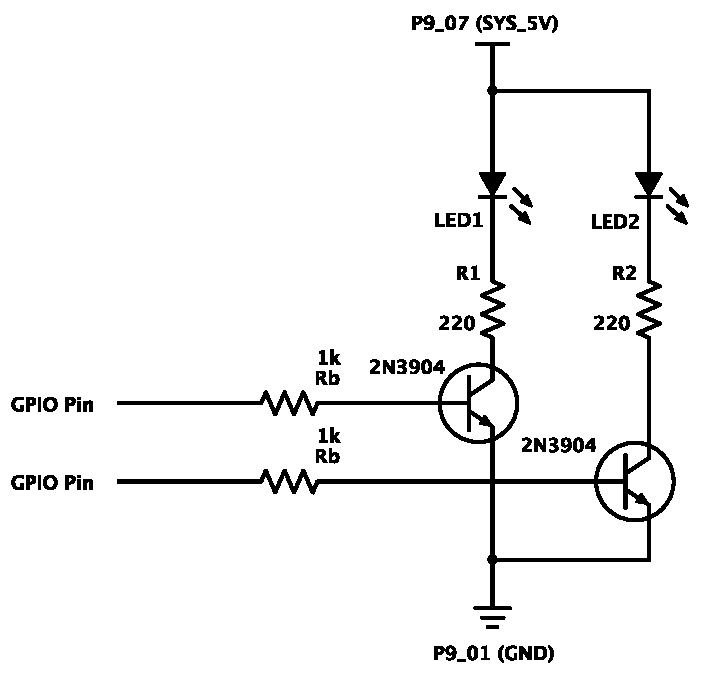
\includegraphics[width=0.5\textwidth]{images/led_circuit}
        \caption{Schematic of SSVEP LED Stimulator}
        \label{fig:bbb_led_schema}
    \end{figure}
    BBB has several General-Purpose Input/Output (GPIO) pins that can be used to communicate with external
    devices and circuits. These pins can be raised HIGH (+3.3v) or LOW (0v)
    using Adafruit BBIO library for Python.
}
\par{
    In order to preserve the portability of the system, we decided to use BBB's
    Input/Output capabilities for LED SSVEP stimulation. A simple digital circuit is designed to
    drive the LEDs using transistors (Figure ~\ref{fig:bbb_led_schema}).
    We had to use transistors to switch the LEDs because BBB can not provide enough current
    through its GPIO pins to light an LED brightly. The transistors rapidly switch
    the LED circuits which can be powered by an external power source. The final
    montage of the stimulator can be seen in Figure ~\ref{fig:bbb_ssvep}.
    \begin{figure}[ht]
    \centering
    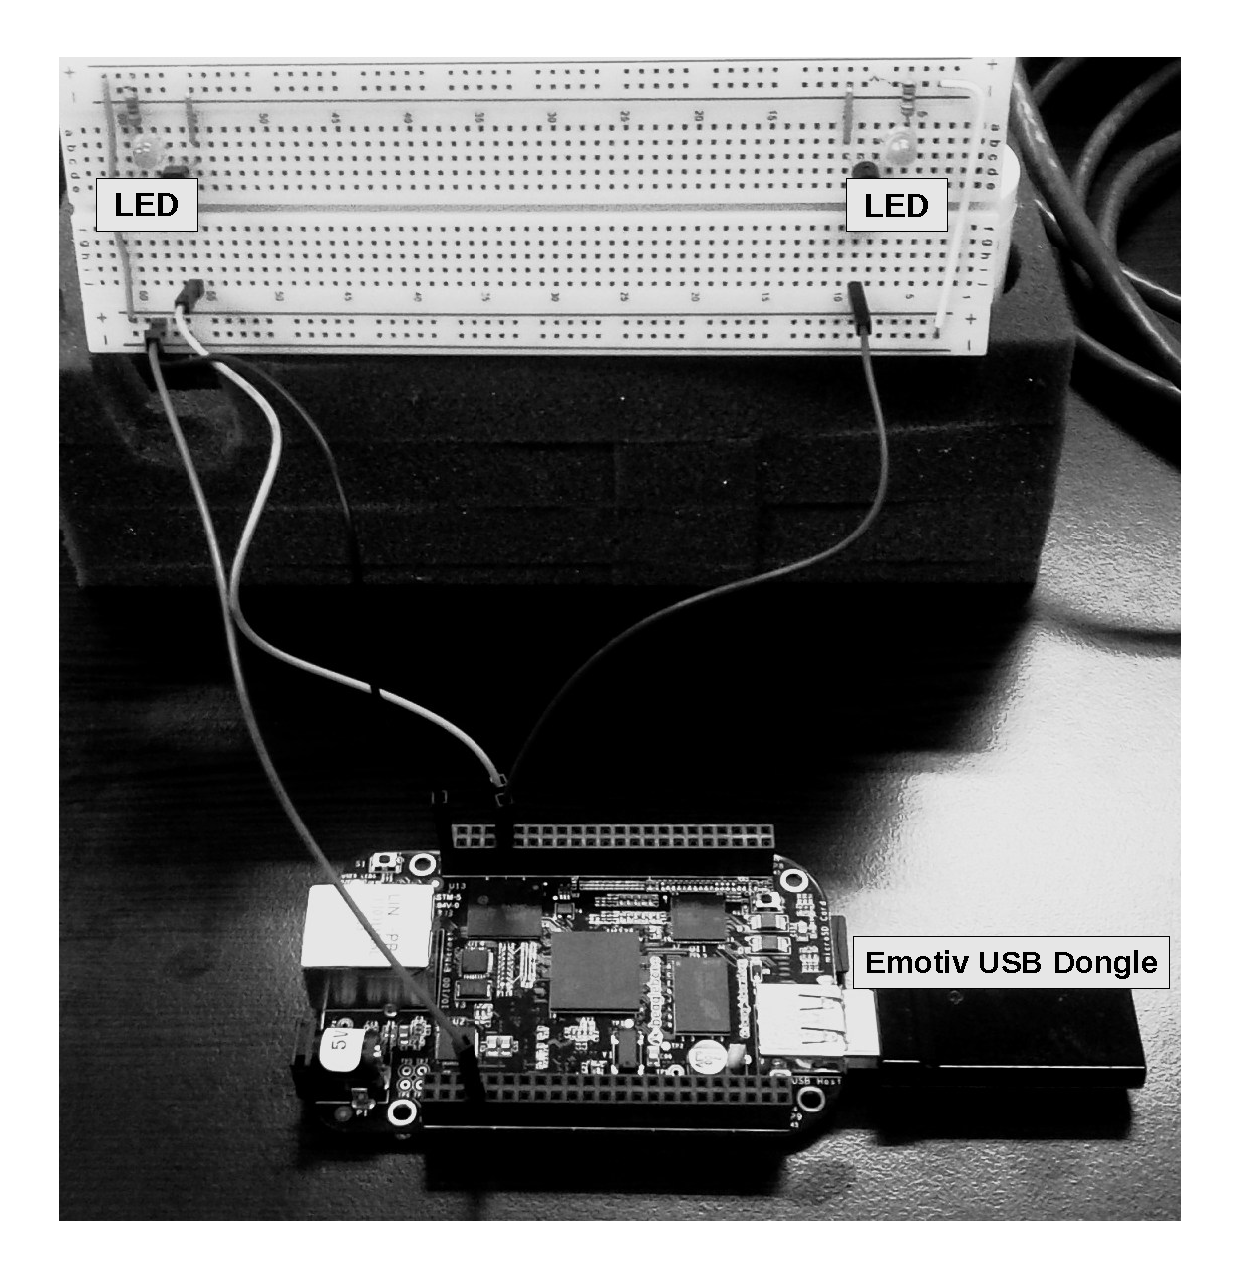
\includegraphics[scale=0.55]{images/bbb_ssvep}
    \caption{LED Montage on BeagleBone Black}
    \label{fig:bbb_ssvep}
    \end{figure}
}

\mysubsubsubsection{SSVEP Software Block}
\par{
    A Python script (\texttt{bbb-bci-ssvepd.py}) is written to manage the external stimulation circuit. We do not
    currently use the PRU for SSVEP stimulation as BBB seems to run good enough
    all of the BCI stack without any issue.
}
\par{
    To start the stimulator, the flickering frequencies, $f_1$ and $f_2$ are passed as command line arguments to the
    script which changes the mode for GPIO pins to \emph{output}, computes
    the triggering periods $T_1$ and $T_2$ for each frequency according to
    the formula $T_i=\frac{1}{2f_i}$ and finally blocks until a signal (namely
    \texttt{SIGUSR1} signal) is sent to it to start the stimulation.
    Once the process receives this signal, it continuously compares the system time and
    previously computed triggering periods to decide whether it is time for
    changing the state of the LEDs or not. The stimulation continues until
    the arrival of a new signal.
}

\mysubsubsection{Signal Processing}
\par{
    The signal processing (SP) block (\texttt{bbb-bci-dspd.py}) creates a UNIX
    socket and waits for new data which will eventually be sent by the EEG acquisition block.
    Once a new chunk of data is received, \texttt{process\_eeg()}
    function is called to process, evaluate and send a control signal
    to the humanoid robot. The SP block then returns to its main loop
    to wait for new data.
}

\mysubsubsection{EEG Acquisition}
\par{
    \begin{figure}[ht]
        \centering
        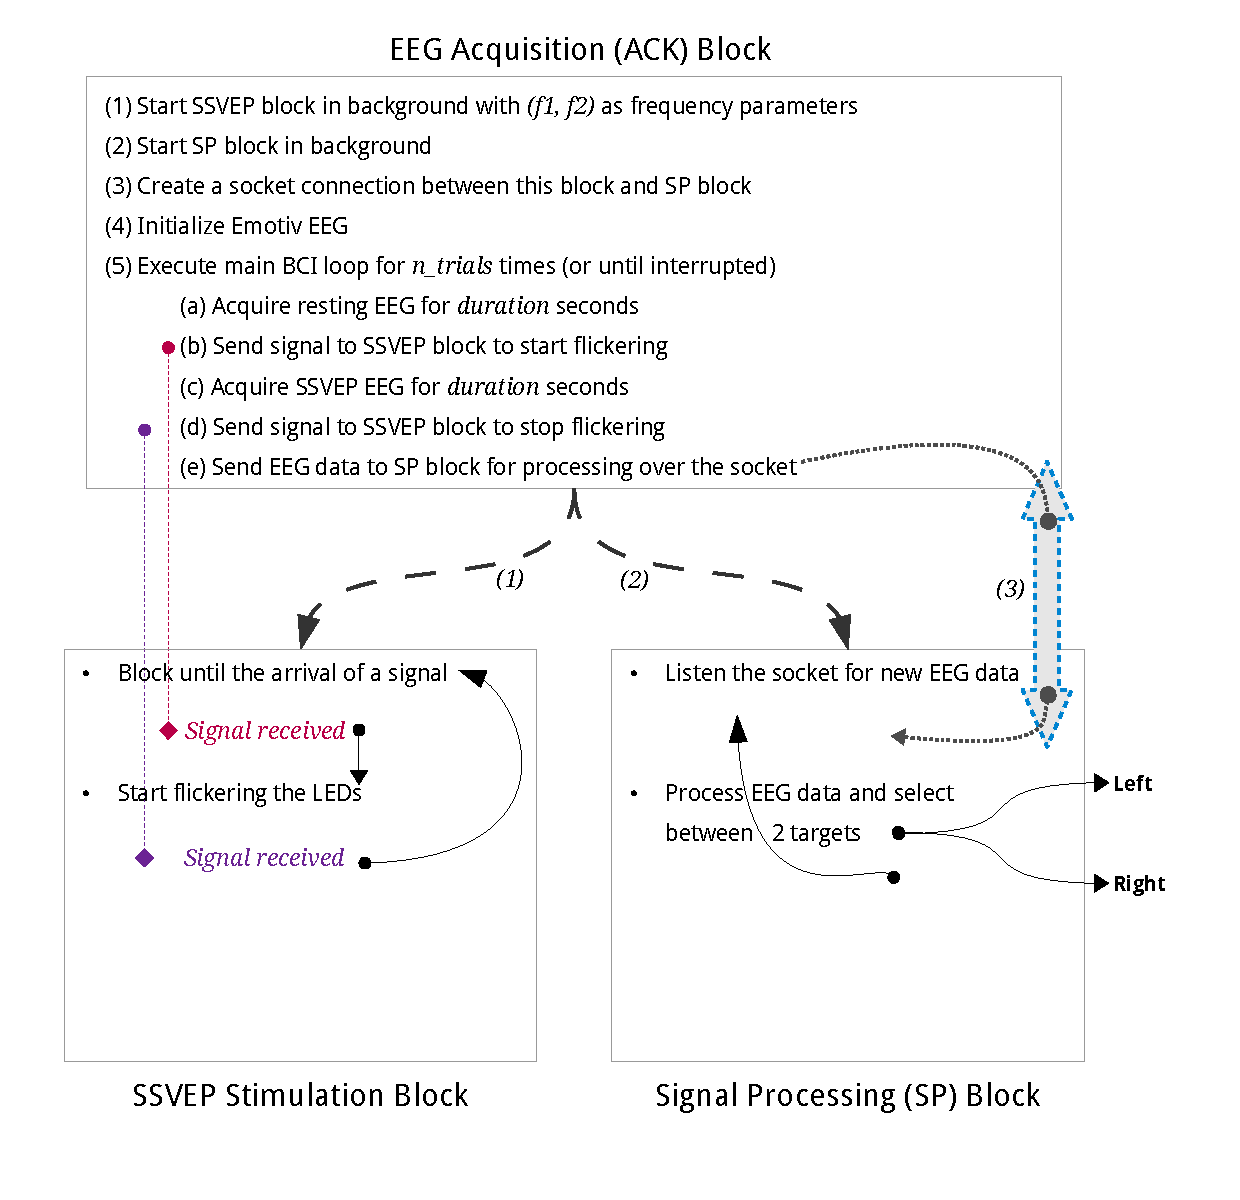
\includegraphics[width=\textwidth]{images/workflow}
        \caption{BCI Workflow}
        \label{fig:workflow}
    \end{figure}
    The EEG acquisition block is actually what manages other blocks and thus
    can be considered as the main entry point to the BCI application. It first
    starts SSVEP block with the desired flickering frequencies, then it starts
    SP block and connects to it through the UNIX socket. After collecting
    some personal information about the subject (Initials, age and sex), it starts the acquisition
    loop which is detailed in Figure ~\ref{fig:workflow}.
}

%%%%%%%%%%%%%%%%%%%%%%%%
%%% Experiment Setup %%%
%%%%%%%%%%%%%%%%%%%%%%%%
\mysubsection{Experimental Setup}

\par{
    We currently tuned the SSVEP stimulator to flicker two green LEDs at
    frequencies $f_1=13Hz$ and $f_2=17Hz$ to represent the left and the right
    arm of the humanoid robot.
}
\par{
    For each run, after activating SSVEP stimulation, 10 seconds of EEG is acquired through the occipital electrodes
    $O1$ and $O2$. The acquired data is then sent to the SP block for signal processing
    and feature extraction.
}
\par{
    Once the EEG data is received by the SP block, it is:
    \nomenclature{FFT}{Fast Fourier Transform}
    \begin{itemize}
        \item Detrended using the \texttt{detrend} method from \texttt{scipy.signal} package
        \item Re-referenced against $O1$ to further filter unwanted EEG components
    \end{itemize}
    The resulting signal is band-pass filtered between $8-45Hz$ before computing
    its frequency spectrum using fast fourier transform (FFT) algorithm.
}
\par{
    For feature extraction, a simple \emph{area under the curve} (AUC) computation is applied on the
    frequency spectrum of the signal near ($\pm1Hz$) the flickering frequencies $f_1$ and $f_2$.
    The AUC is then used to decide the LED frequency attended by the user to
    choose between 2 states representing the arms of the humanoid robot.
    The relevant command is finally sent to the robot to realize the actual
    movement of the selected arm.
}
% FIXME Results
%\mysubsection{Results}
%\par{
%}

%%%%%%%%%%%%%%%%
%% CONCLUSION %%
%%%%%%%%%%%%%%%%
\clearpage
\vspace*{-0.35cm}
\mysection{CONCLUSION}
\par{
    In this study, a proof of concept, portable and embedded SSVEP BCI system to demonstrate
    humanoid robot control is presented. A cheap, single-core embedded computer is used
    along with a consumer grade, battery-powered, wireless and affordable EEG headset
    to reach maximum portability and minimum cost.
}
\par{
    All software blocks regarding stimuli presentation,
    EEG acquisition, signal processing and robot control are implemented in Python and
    they are all running in parallel without any jitters and delays. This is
    an important achievement to prove that the usage of embedded computers in BCI
    research is possible.
}

%%%%%%%%%%%%%%%%
%% REFERENCES %%
%%%%%%%%%%%%%%%%
\clearpage
\vspace*{-0.35cm}
\bibliographystyle{apalike}
\phantomsection
\thispagestyle{empty}
\addcontentsline{toc}{section}{References}
\bibliography{ThesisLibrary}

%%%%%%%%%%%%%%
%% APPENDIX %%
%%%%%%%%%%%%%%
%\clearpage
%\cfoot{}
%\vspace*{-0.35cm}
%\thispagestyle{empty}
%\section*{Appendix}
%\addcontentsline{toc}{section}{Appendix}
%\vspace*{6pt}
%
%\subsection*{SSVEP Stimulator}
%
%\renewcommand{\baselinestretch}{1.0}
%\lstinputlisting[language=Python, basicstyle=\footnotesize\ttfamily,
%                 breaklines=true, tabsize=2,
%                 showspaces=false, keepspaces=true, showstringspaces=false,
%                 keywordstyle=\color{blue},
%                 commentstyle=\color{gray},
%                 stringstyle=\color{purple},
%                 ]{code/bbb-bci-ssvepd.py}
%\newpage
%\subsection*{EEG Acquisition Block}
%\lstinputlisting[language=Python, basicstyle=\footnotesize\ttfamily,
%                 breaklines=true, tabsize=2,
%                 showspaces=false, keepspaces=true, showstringspaces=false,
%                 keywordstyle=\color{blue},
%                 commentstyle=\color{gray},
%                 stringstyle=\color{purple},
%                 ]{code/bbb-bci-acquire.py}

%%%%%%%%%%%%%%%%%%%%%%%%%
%% BIOGRAPHICAL SKETCH %%
%%%%%%%%%%%%%%%%%%%%%%%%%
\clearpage
\cfoot{}
\vspace*{-0.35cm}
\thispagestyle{empty}
\section*{Biographical Sketch}
\addcontentsline{toc}{section}{Biographical Sketch}
\vspace*{6pt}
\par{
    Ozan Çağlayan was born on September 11, 1985 in Istanbul, Turkey. After graduating from Saint-Joseph French High School in 2004,
    he began studying Computer Engineering at Galatasaray University. In 2007, he spent a semester at Université Joseph Fourier (Grenoble/France) as part of Erasmus Exchange Programme.
    In September 2007, he became a part-time software developer of Pardus Linux, the national Linux-based operating system project
    managed by The Scientific and Technological Research Council of Turkey (TUBITAK). After receiving his Bachelor of Science in 2008, he continued working for Pardus Linux project until January 2012.
    Since October 2012, he is working as a research assistant at Galatasaray University.
}
\clearpage

\end{document}
